%*******************************************************************************
%*********************************** First Chapter *****************************
%*******************************************************************************

\chapter{Plastic deformation}  %Title of the First Chapter
\label{chap:plastic_deformation}

\epigraph{I have ventured to call them dislocations}{A.E.H. Love}




\graphicspath{{plastic_deformation/Figs/}}

Plastic deformation or plasticity is the process of permanently altering the shape of a solid body under the influence of an applied external force. Indeed under the application of a large enough force and if cracking can be suppressed, for example by applying a confining pressure, most materials will plastically deform. Though a range of mechanisms for plastic deformation exist in crystals by far the most widespread is dislocation glide. Glide was first observed in 1867 \cite{Reusch1867} and was studied formally as early as 1899 \cite{Ewing1899,Ewing1900}. However it was not known or even proposed that dislocations, linear defects in a crystal structure, mediate plastic flow by moving over rational crystallographic planes \cite{Kelly2012ch7}.

If the process of dislocation glide cannot occur then a material is usually {brittle} and will fail by fracture or cracking, while if dislocation glide can occur a material is usually {ductile} and will fail by yielding. Brittleness vs ductility of a material is not a fixed property but will depend on the stress state and the temperature. If sufficiently high hydrostatic pressure is applied then even materials like sapphire will undergo plastic flow \cite{Bridgman1947}. At high temperatures, thermal activation can enable glide to occur in materials that are brittle at lower temperatures, with many materials known to exhibit ductile to brittle transition temperatures, for example body-centre iron, titanium carbide and olivine among many others   \cite{Kelly2012ch7,frost1982,Rowcliffe1971,Darot1985}.

Dislocation motion is of much practical importance in crystalline materials. In many metals, particularly those with a face-centred cubic structure such as copper or aluminium, dislocation motion must be hindered to achieve sufficient strength for use as an engineering material. Much of physical metallurgy is the study of the microstructural features that affect dislocation motion and their genesis in materials processing or alloy composition.

In other materials the crystal structure itself provides such a large barrier to motion that almost no plastic deformation is possible and these materials usually fail by brittle fracture. This is true of many non-metallic materials widely used as protective coatings or as functional materials in devices. Fracture is often the life limiting factor for these materials, thus if their toughness were increased by making plastic flow were easier their lifetime might be extended. 

Even in some metallic materials with comparatively simple crystal structures plastic flow is limited not by microstructural features but by the inherent resistance of the crystal structure to the motion of dislocations. This is common in body-centred cubic metals, tantalum and niobium at room temperature and iron at lower temperatures \cite{Christian1983,Weinberger2013}, but also in the face-centred cubic metal iridium; the low mobility of dislocations in iridium is at least partly responsible for its tendency to fail by cleavage \cite{Panfilov2001}. The ductile to brittle transition in many metals is due to the lattice resistance, notably iron in its body-centred form becomes brittle at low temperatures. This resulted in the failure of the Liberty ships during the second world war in the cold waters of the North Atlantic. Originally thought to be due to high stresses caused by the welding technique used to join the steel, it was Constance Tipper who showed that it was the lack of plastic flow around the crack tip that enabled for the catastrophic failure of entire ships to occur \cite{Cottrell1997}. 

Thus there is a great motivation to understanding the inherent resistance to dislocation flow in a crystal structure, or \emph{lattice resistance}, and in being able to alter that lattice resistance and thereby introduce a degree of toughness to otherwise brittle phases.



\section{Dislocations}  
\label{sec:dislocations}


Dislocations are line defects in crystals that are important, amongst other reasons, because they are responsible for plastic deformation. Though the character of dislocations can vary in a continuous fashion there are two limiting cases: Edge dislocations can be introduced to a perfect crystal by the introduction of an extra half plane of atoms, the termination of this half plane is the dislocation, see \autoref{fig:Edge_disloc_loop}; screw dislocations are formed by shearing a region of crystal such that the lattice planes form a helix, the centre of the helix is then the dislocation, this is shown in \autoref{fig:screw_disloc}. Mixed dislocations have some of the character of both these end members.



\begin{figure}
\centering

\begin{subfigure}{0.4\textwidth}
\centering
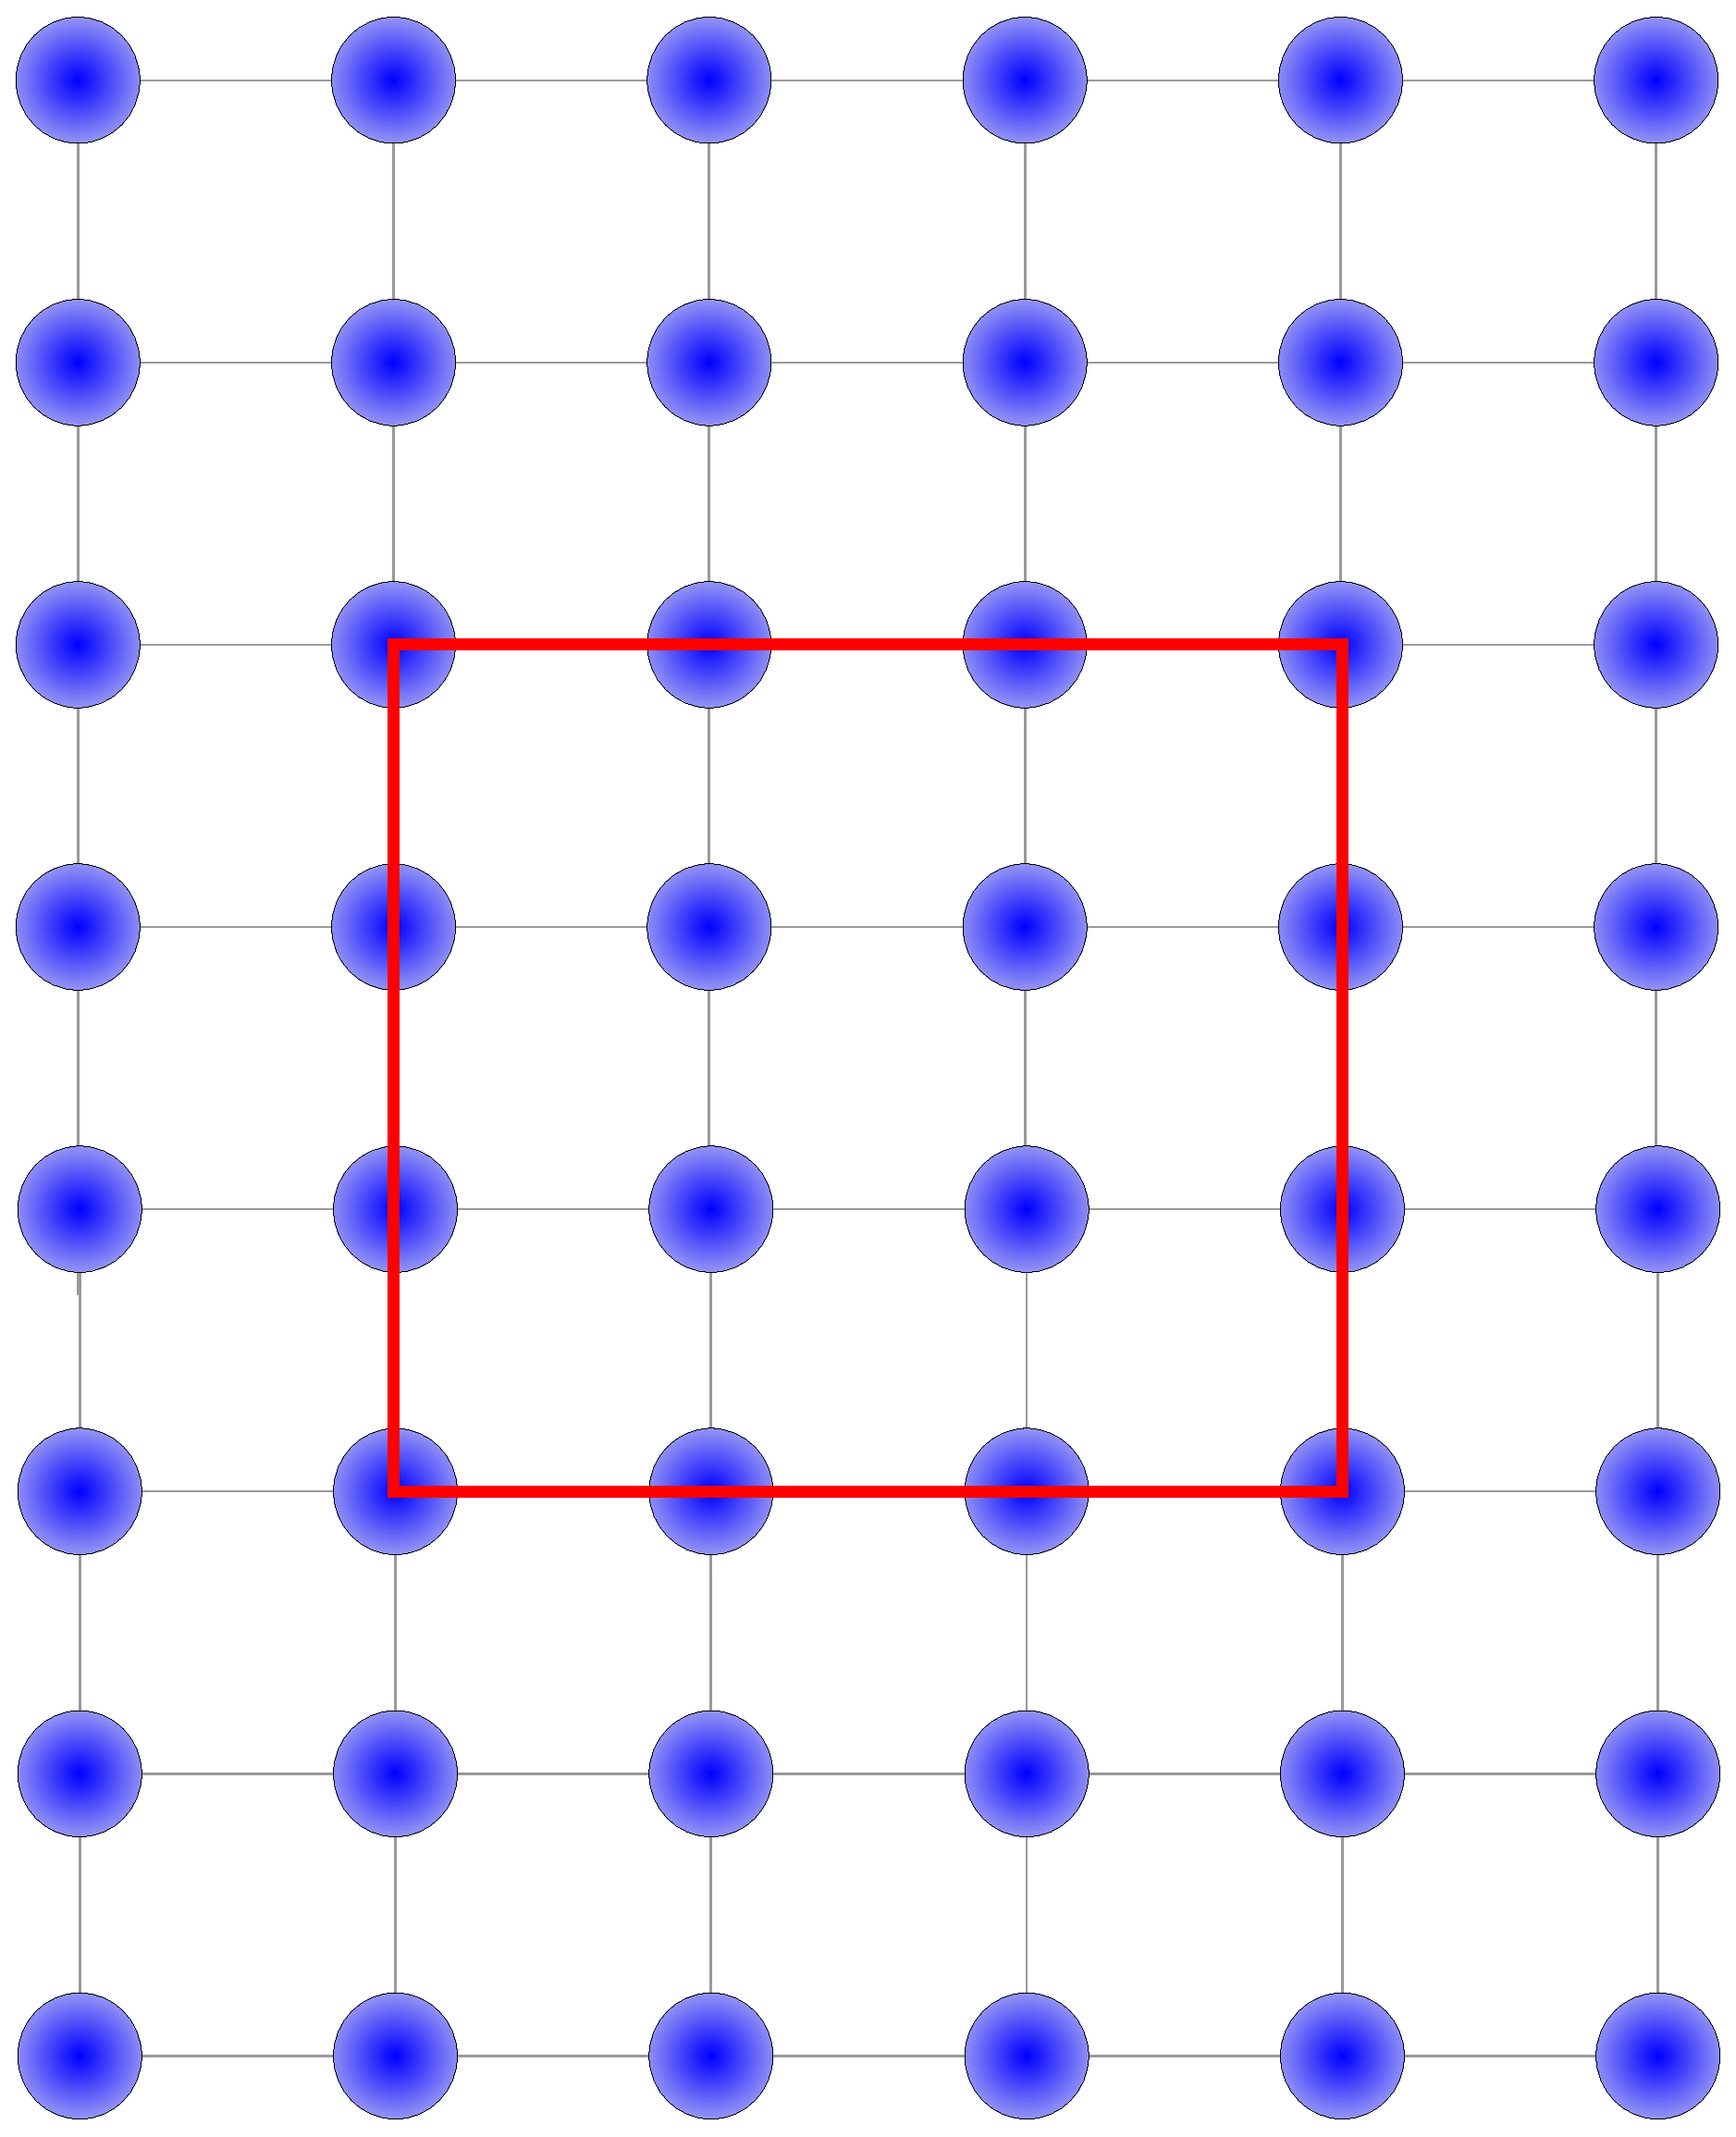
\includegraphics[height=2.5in]{Perfect_crystal_loop}
\caption{A perfect crystal with a complete circuit shown in red.}
\end{subfigure}
\begin{subfigure}{0.4\textwidth}
\centering
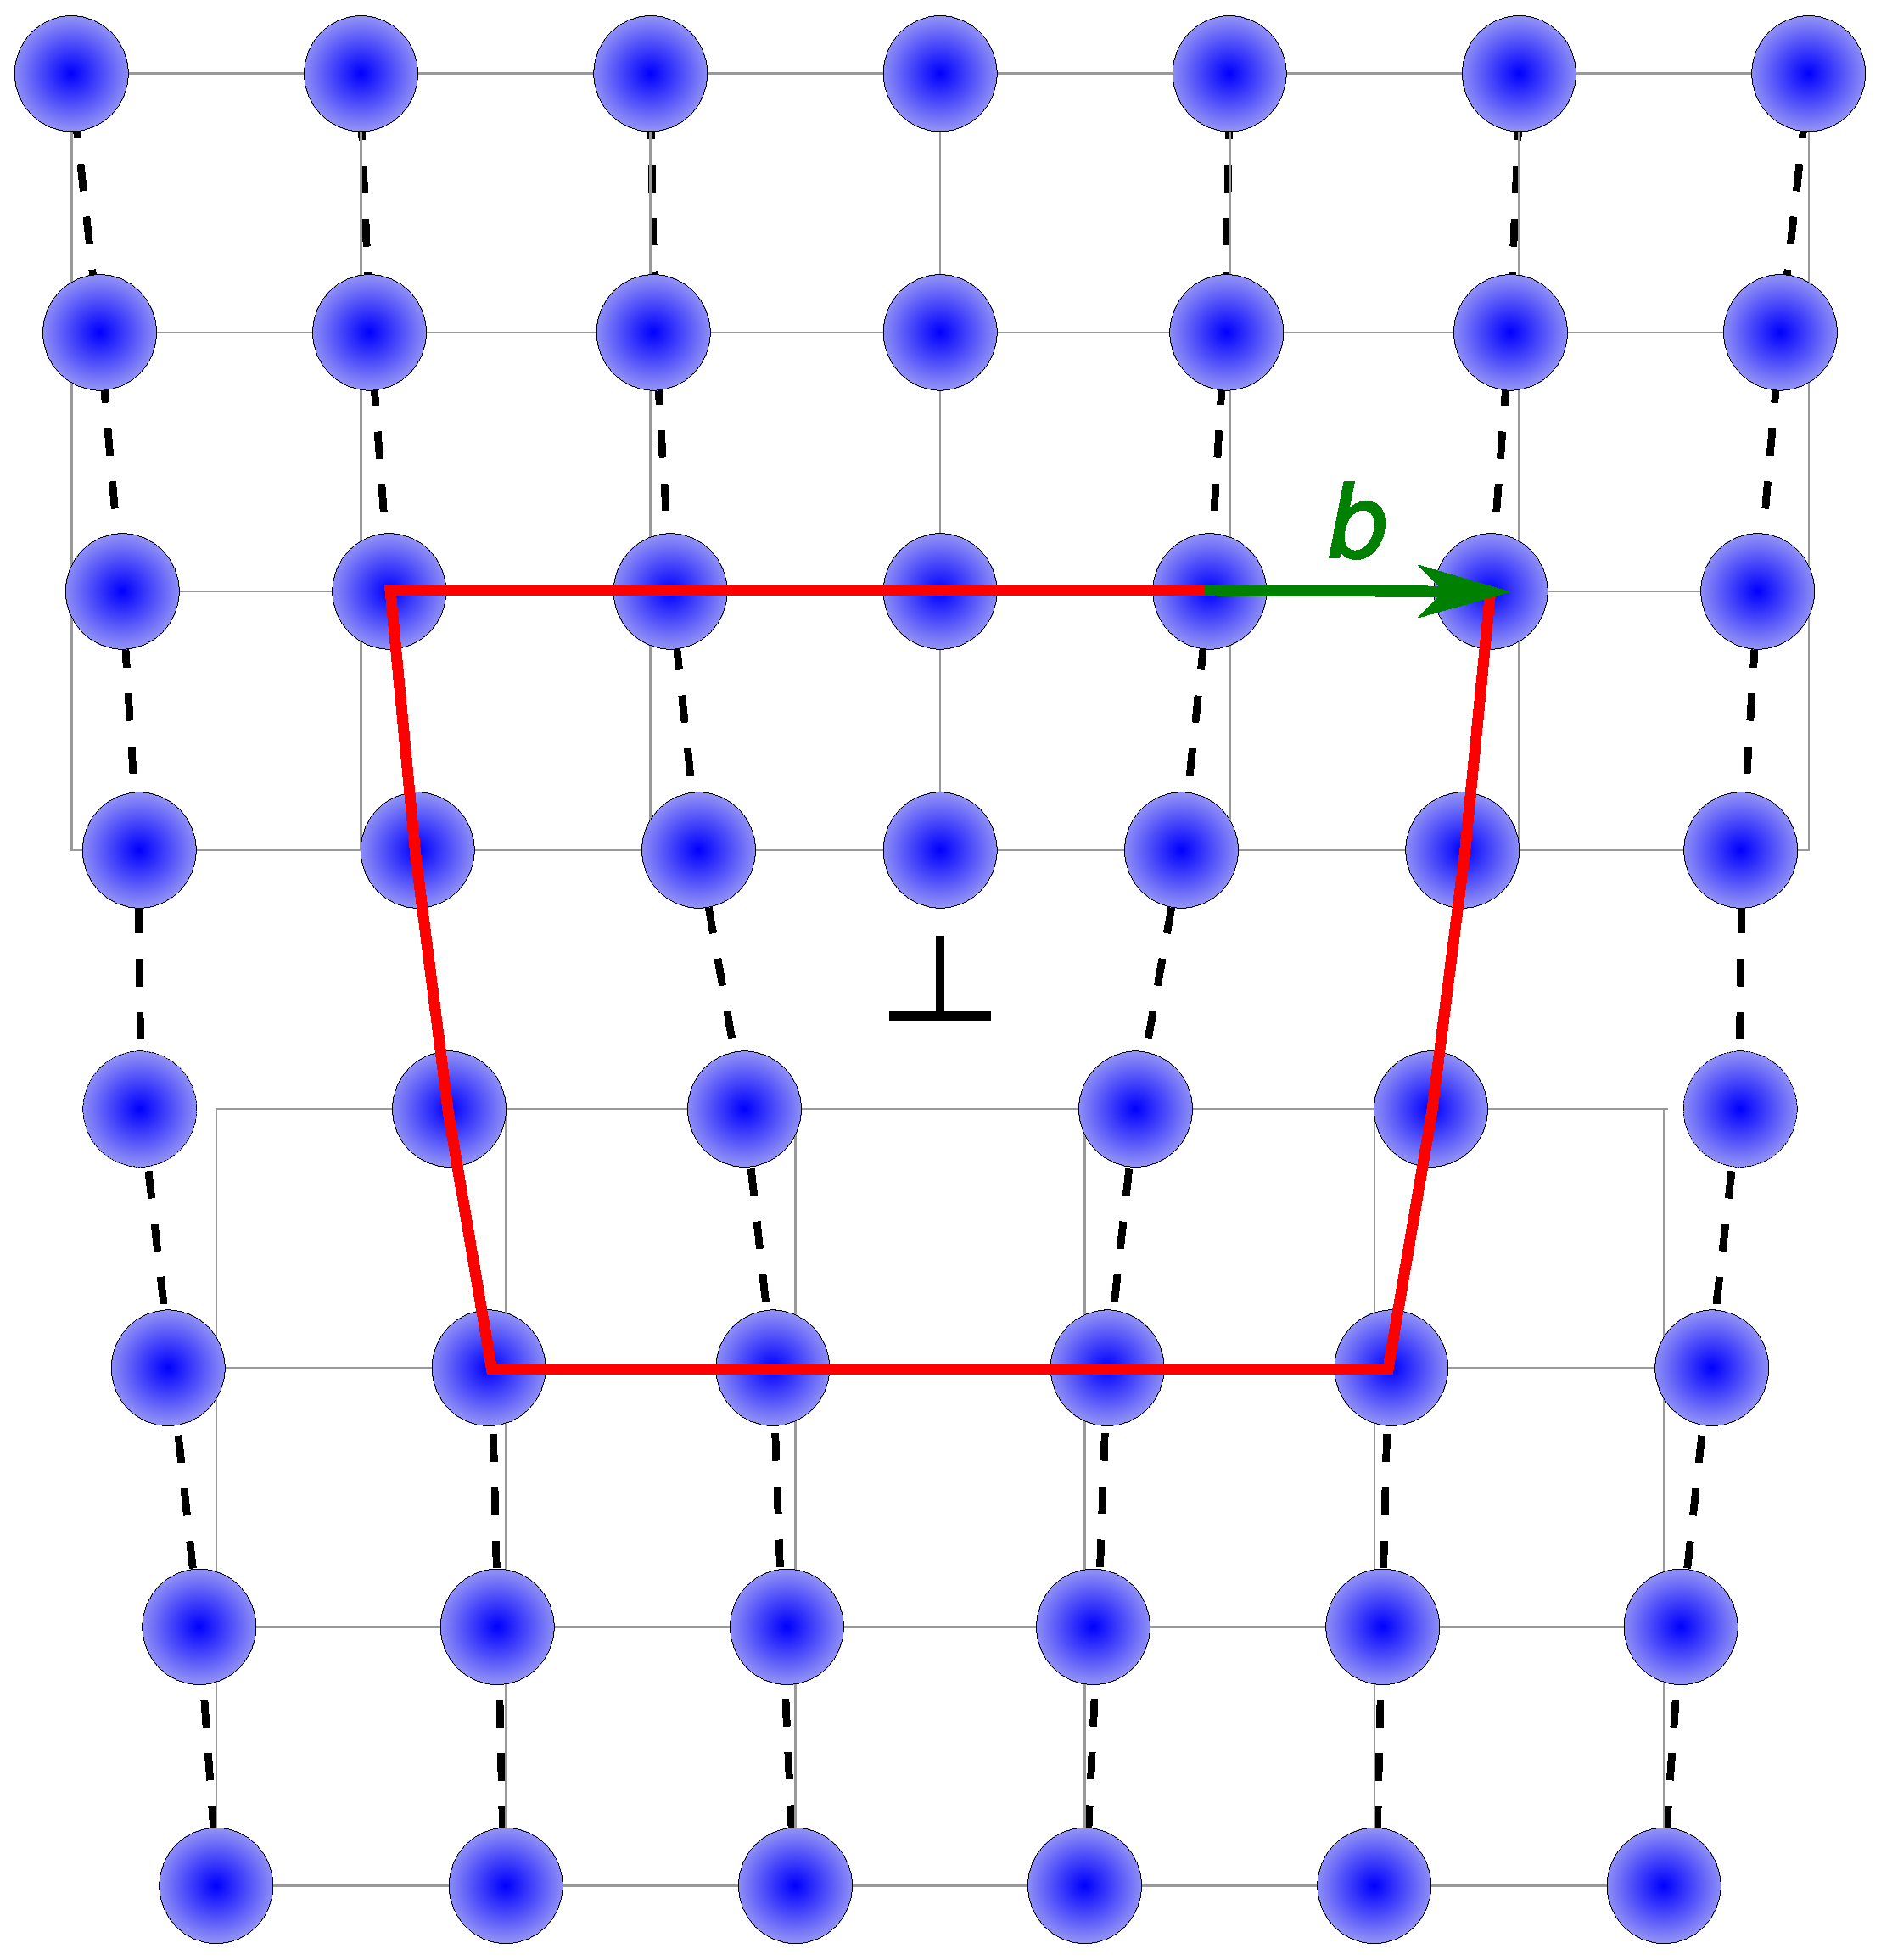
\includegraphics[height=2.5in]{Edge_Dislocation_loop}
\caption{An edge dislocation with an incomplete circuit. \label{fig:Edge_disloc_loop}}
\end{subfigure}

\caption{Inserting a half plane of atoms which terminate in a dislocation and a Burgers circuit to show the Burgers vector. \label{fig:burgers_loops}}

\end{figure}

\begin{figure}
\centering
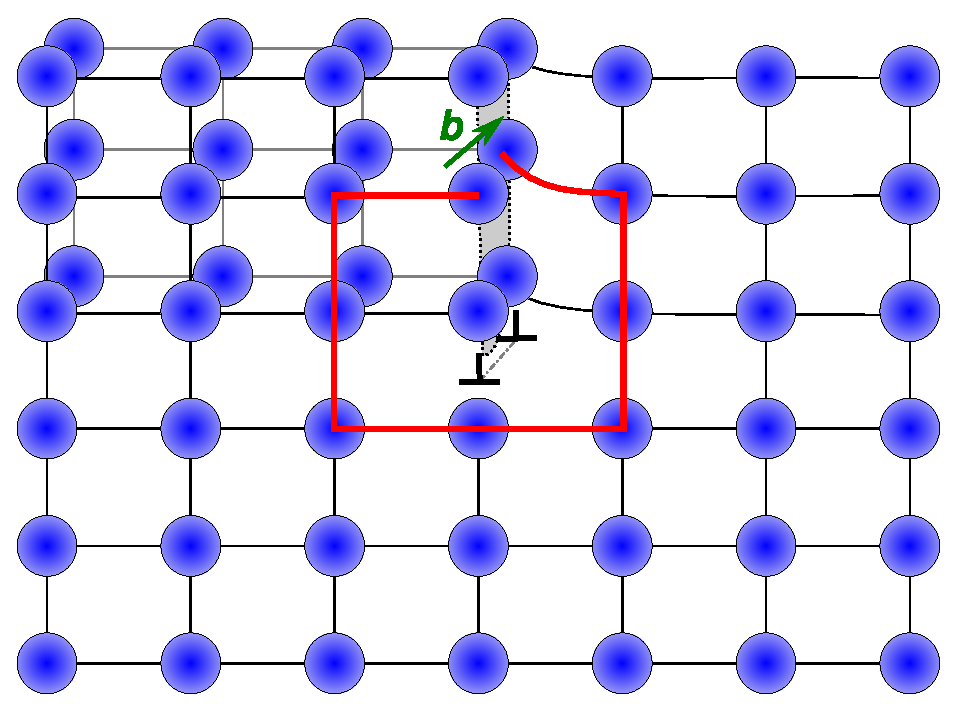
\includegraphics[width=0.7\textwidth]{screw_disloc_loop}
\caption{Schematic of a screw dislocation with a Burgers loop formed in a similar way to \autoref{fig:burgers_loops}. The displacement is parallel to the dislocation line in contrast with edge dislocations. The atomic positions are not relaxed, the displacements being concentrated unphysically into one half plane. \label{fig:screw_disloc}}
\end{figure}




Dislocations can be described in terms of a slip direction, a line direction and a slip plane. The slip direction is simply the direction parallel to the Burgers vector, this is the relative displacement caused by the passage of a dislocation through a region of crystal. The identification of the Burgers vector is done with a Burgers loop, a loop comprised of steps between nearest neighbours is defined that would be closed in a perfect crystal is defined. The same set of steps is undertaken in a dislocated crystal and the loop is no longer closed and the displacement vector between the endpoints is the Burgers vector. This is shown for an edge dislocation in \autoref{fig:burgers_loops}, where the Burgers vector is perpendicular to the line vector, and a screw dislocation in \autoref{fig:screw_disloc}, where the Burgers vector is parallel to the line vector. The line direction can and does vary along the length of the dislocation but is simply the line defined by the defective region of crystal. The slip plane is the crystallographic plane in which the dislocation can move and must contain the slip direction and line direction; where the line and the slip directions are not parallel the slip plane is defined by these two vectors, but for screw dislocations which have the slip direction and line directions parallel the plane is not so constrained, instead the possible slip planes are those that allow easy movement, i.e. lower forces or smaller energy changes, and depending on the crystal symmetry there may be several. This allows screw dislocations to change the plane they are moving in, a process known as cross slip \cite{Hirth_Lothe1982intro}.

Real dislocations are not neat and instead of lining up with convenient crystallographic axes will curve and bend. This usually gives rise to a mixed and varying character of dislocation with the Burgers vector neither parallel nor perpendicular to the line vector. These mixed dislocations are usually described as the sum of edge and screw components.

There are conventions about the sign of dislocations, taking line vectors into or out of the page and defining the sense of Burgers loops and the Burgers vector defined from the finish to the start etc. Given that the symmetry of most of the crystals of interest is high enough to ensure that all these choices are usually arbitrary the only thing that will be highlighted here is that if the sense of a dislocation is reversed then its stress/strain field will reverse in sign. Hence oppositely signed dislocations attract to lower the stored elastic energy and potentially to annihilate line length, while like-signed dislocations will repel to lower the elastic stored energy.



\FloatBarrier

\subsection{Historical overview}


In the early twentieth century there were many observations of real world materials strengths that could not be reconciled with the theoretical shearing strength of a perfect plane of atoms. Indeed for a long time this was neglected because, as \citet{gordon1991} puts it:
\begin{quote}
``Until about 1934 the Establishment explanation of these phenomena was remarkably unconvincing and seems to have reflected mainly a desire not to be asked embarrassing questions.''
\end{quote}

In 1934 the edge dislocation was proposed by \cite{orowan1934i,Orowan1934ii,Orowan1934iii}, \citet{Taylor1934}, and \citet{polanyi1934} to explain the discrepancy between the ideal strength of crystal and the observed strengths of real materials. It was around this time that work undertaken by \citet{Volterra1907} and others, particularly \citet{love1920}
on elastic behaviour of homogeneous isotropic continua was related to plastic flow of crystalline materials, idealised dislocations in elastic continua are termed Volterra dislocations. By the end of the decade \citet{burgers1939} had described screw dislocations. 

It was not until the 1950s that experimental evidence for the existence of dislocations was produced; the initial evidence was growth surfaces of single crystals, preferential etching of a crystalline material at dislocations and x-ray studies of arrays of dislocations in the bulk \cite{Forty1954}. 

\citet{Frank1949} predicted, in 1949, that a step could terminate by the intersection of a dislocation with a free surface, or conversely a dislocation intersecting with a free surface would necessarily create a step; these weere observed soon after in 1950 by \citet{Griffin1950}. Preferenctial etching of dislocations was observed by \citet{horn1952holes} who matched the configuration of etch pits with the pre-existing surface growth features that arise from screw dislocations. The effect of plastic work and subsequent recovery on Laue spots (the xray beams diffracted by a single crystal) provide evidence of arrays of dislocations. The process is described by \citet{Cottrell1949}: Initially sharp Laue spots exist in a perfect crystal. Plastic work smears the spots by introducing a homogeneous distribution of dislocations and the spots then split into distinct sharp spots during recovery as dislocations align into arrays that form sub-grains with small misalignments across the new low angle grain boundaries.


An edge dislocation was first imaged in 1956 by \citet{Menter1956} in platinum phthalocyanine. The large organic complex with a platinum atom at the centre produces widely spaced rows of platinum atoms suitable for imaging with transmission electron microscopy.




\subsection{The stress required to move a dislocation}

Though mathematical descriptions of dislocations in isotropic elastic continua date back to 1907 \cite{Volterra1907} the energies and forces around dislocations in crystalline lattices and the  was not considered until much later. In 1940 \citet{Dehlinger1940} and \citet{Peierls1940}. The former presented the application of the Frenkel-Kontorova model, a one dimensional array of balls connected by springs on a periodic potential/substrate, to approximate a dislocation.

The latter, Rudolph Peierls, was one of the physicists working during the advent of quantum mechanics and most of his work was in that field, however during his education he received a grounding in classical physics at Arnold Sommerfeld's lectures in Munich and so it was that he was suitably equipped when presented with the problem of dislocation motion by Egon Orowan; as Peierls remarked he knew nothing about dislocations but he did know classical elasticity \cite{Edwards1996}.


Peierls presented the first formal solution for the energy changes as a dislocation moves in a rather short note \cite{Peierls1940} and the idea was extended by \citet{Nabarro1947}. The model is remarkably simple; consider two semi-infinite perfect crystals with their lattice aligned but some initial misalignment between them as shown in \autoref{fig:semi_infinite_crystals}. We can join them along what will become the slip plane. An edge dislocation is formed where the energy of the system is lowered by displacing atoms from their initial positions to localise the misalignments around the dislocation core, usually taken to be the origin. I.e. when the energy of a planar defect is higher than that of the linear defect and dislocation will form.



\begin{figure}
\centering

    \begin{subfigure}{0.4\textwidth}
        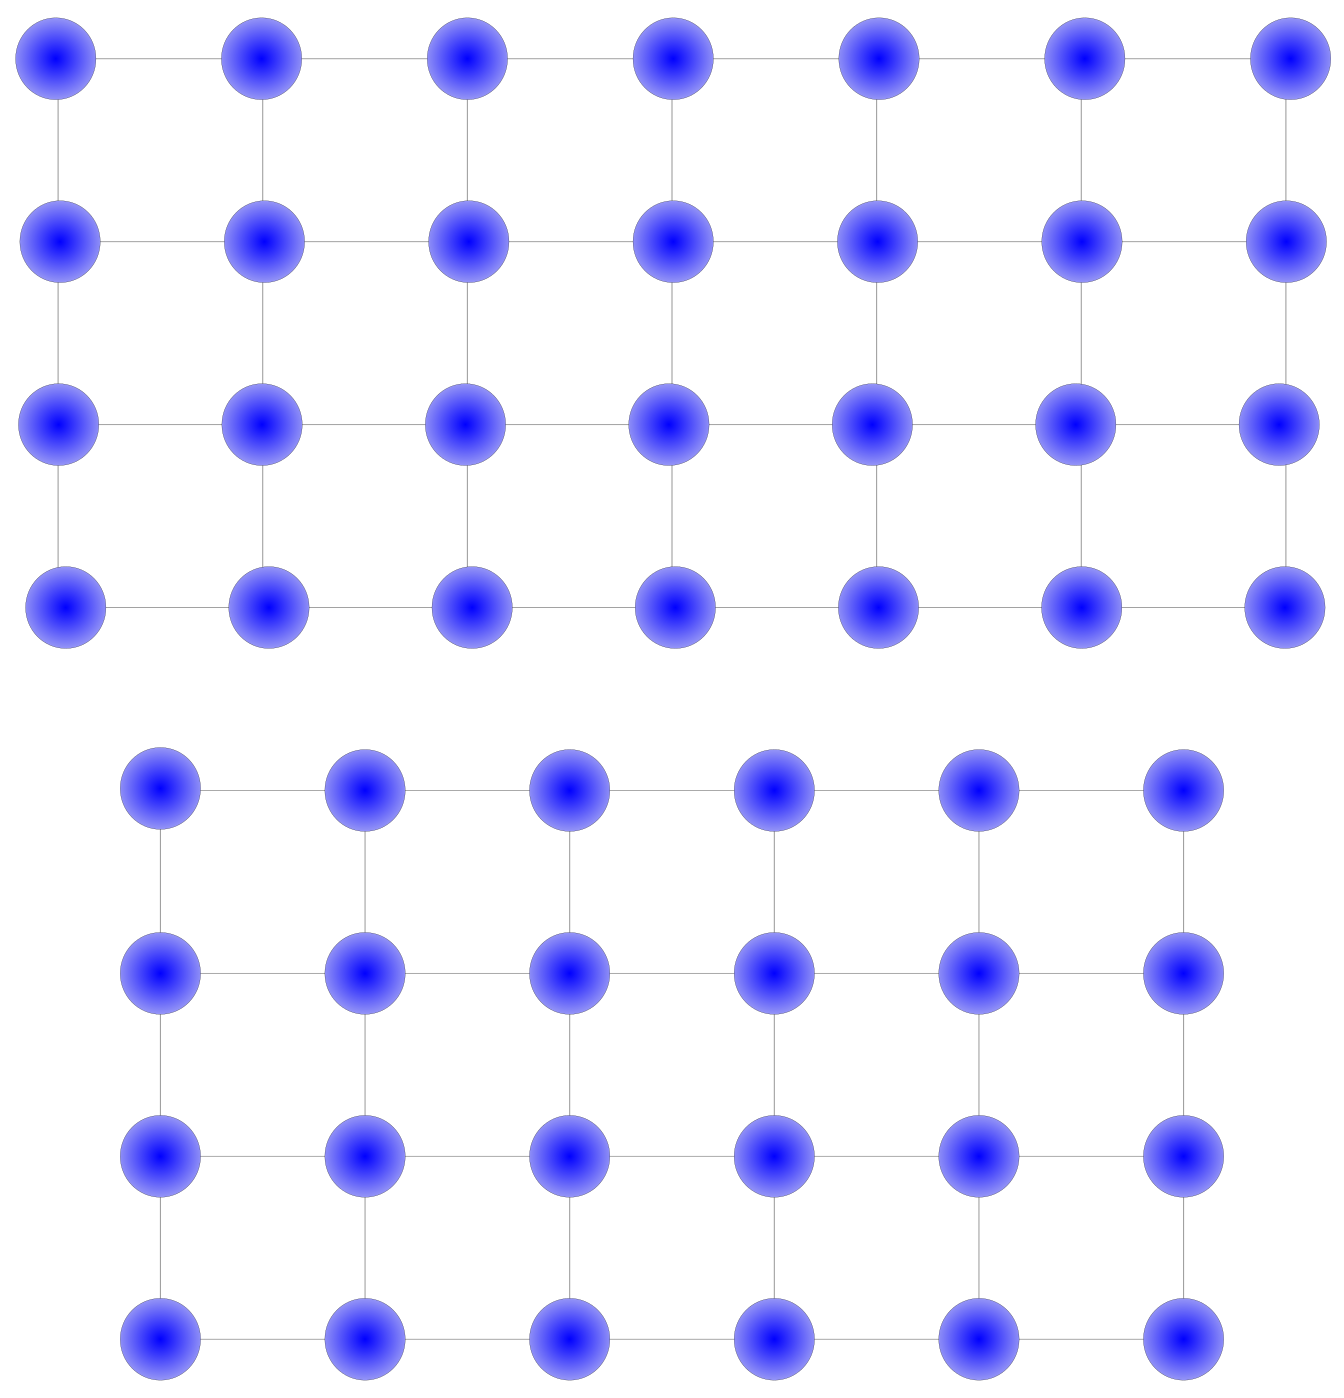
\includegraphics[width=\textwidth]{Half_crystals}
        \caption{Two semi-infinite crystals \label{fig:semi_infinite_crystals}}
    \end{subfigure}

    \begin{subfigure}{0.4\textwidth}
        \includegraphics[width=\textwidth]{Edge_Dislocation}
        \caption{A schematic edge dislocation\label{fig:joined_half_crystals}}
    \end{subfigure}

    \caption{Schematics showing the creation of an edge dislocation in a simple square lattice by the joining of two misaligned half crystals. \label{fig:edge_disloc}}
\end{figure}

\begin{figure}
\centering
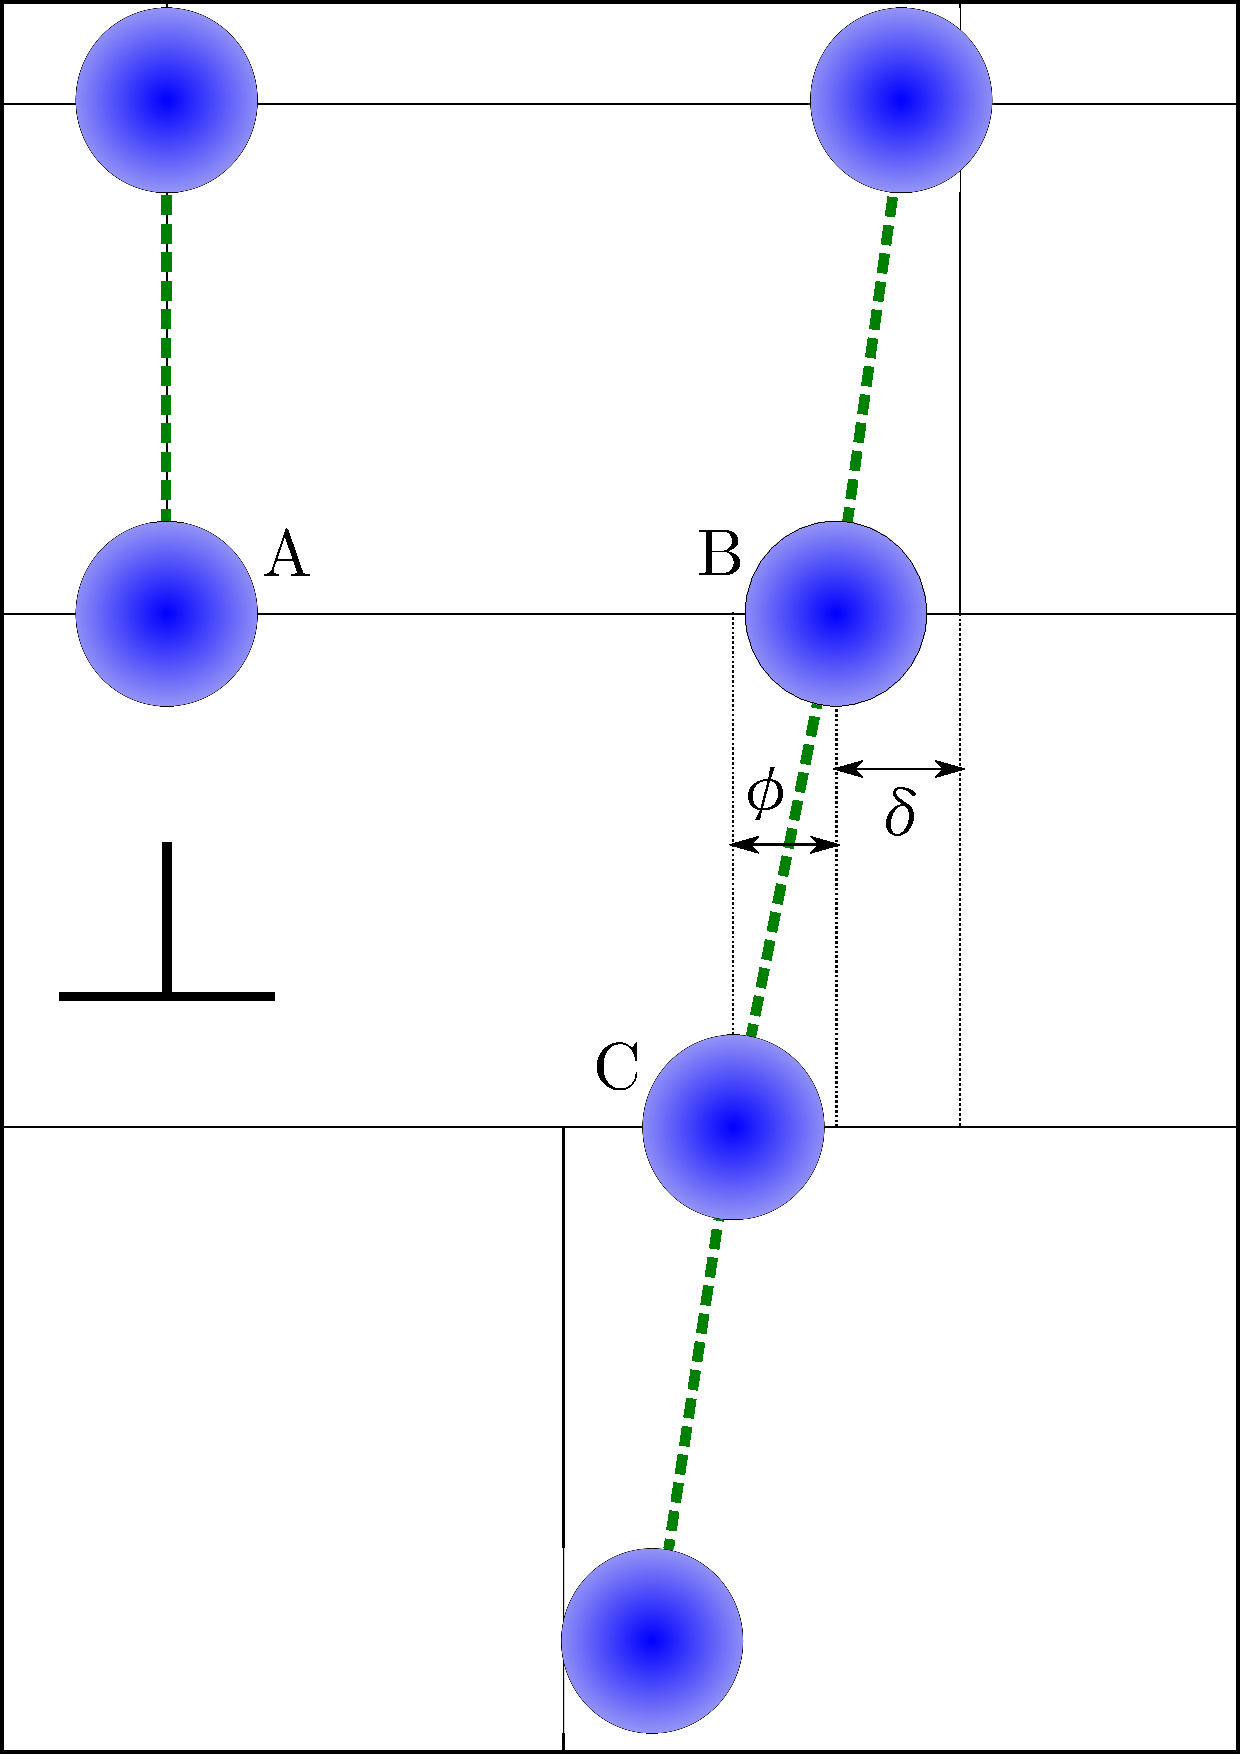
\includegraphics[width=0.6\textwidth]{peierls_model_detail}

\caption{Detail of the local displacements around the dislocation core. $\delta$ is the extension of the bond parallel to the slip plane between atoms A and B, while $\phi$ is the misalignment of the bond across the slip plane between B and C.\label{fig:detail_of_peierls}}
\end{figure}

Atomic configurations that form a dislocation are generated by by applying a displacement field to the atoms immediately above and below the slip plane, $u(x)$ and $u'(x)$ respectively. The Peierls model then estimates the energy of the configuration by considering two restoring forces generated by the atomic arrangement. The detail is show in \autoref{fig:detail_of_peierls}. Firstly the bonds parallel the slip plane will be either extended or contracted, for example the bond between atom $A$ and $B$ has been contracted by the amount $\delta$, this will tend to oppose the concentration of misalignments to the core and is zero in the case of no displacements from the initial positions. Secondly the misalignment of bonds across the slip plane, the bond between atom $B$ and $C$ is misaligned by a lateral distance of $\phi$. This misalignment energy will tend to favour the concentration of the misalignments to the core and is a maximum in the case of no displacement from the initial position.

Peierls made the assumption that the displacements vary slowly with position, i.e. that the dislocation is very wide. This means that the strain in the slip plane (i.e bonds like $\overrightarrow{AB}$ in \autoref{fig:detail_of_peierls}) experience only small strains. The energy associated with these \emph{in-plane} strains are then described  by the application of the displacement field to the surface of two semi infinite elastic continua. 
The \emph{misalignment} energy of bonds across the slip plane (bonds like $\overrightarrow{BC}$ in \autoref{fig:detail_of_peierls}) is assumed to be a periodic function, specifically a simple sinusoidal variation is taken to be the form of the misalignment potential:

\begin{equation}
U_{mis} = C \sin \left(\frac{2\pi [u(x) - u'(x)]}{d} \right)
\end{equation}













%%%%%%%%%%%%%%%%%%%%%%%%%%%%%%%%%%%%%%%%%%%%%%%%%%%%%%%%%%%%%%%%%%%%%%%%%%%%%%%%%%%%%%


%
%
%
%
%   Sort out this Frenkel stuff
%
%
%
%
%
%


%%%%%%%%%%%%%%%%%%%%%%%%%%%%%%%%%%%%%%%%%%%%%%%%%%%%%%%%%%%%%%%%%%%%%%%%%%%%%%%%%%%%%%



The constant, $C$, has to be chosen appropriately but can be found by assuming linear elasticity holds at small strains. \citet{Frenkel1926} derived a similar sinusoidal function for the stress to form a stacking fault:










\begin{equation}
\tau_{fault} = \tau_{\text{theory}} \sin \left( \frac{2\pi \phi}{b} \right)
\end{equation}

The energy of the dislocation is the sum of all these contributions. There will be a configuration that is a minimum in the total energy where the in-plane forces widening the dislocation balance the misalignment forces that drive it to be narrower. This gives rise to a size, or width, of a dislocation. The width of the dislocation is defined as the distance from the core at which the misalignment across the slip plane is half its maximum. Peierls calculated this for an isotropic elastic solid and accounting for only the atomic planes immediately adjacent to the slip plane and found it to be 

\begin{equation}
w = \frac{d}{1-\nu}
\label{eqn:width_isotropic}
\end{equation}
where $d$ is the plane spacing across the slip plane and $\nu$ is the Poisson ratio.

The stress required to move a dislocation can be calculated from the maximum energy \emph{gradient} as the dislocation is displaced. Since the in-plane strains have a continuous definition in this model the displacement of the dislocation has no effect and the in-plane strain energy does not change. The energy changes therefore depend only on the misalignment energy of bonds across the slip plane and the energy of all the atoms away from the slip plane re neglected.

Peierls gave the critical stress, the \emph{Peierls Stress}, for an isotropic elastic material in terms of the ideal shear strength as calculated for uniform slip and accounting for only the interactions between the first plane either side of the slip plane, as


\begin{equation}
\frac{\tau_p}{\tau_{ideal}} = \frac{4 \pi}{1 - \nu} (5.8 - \log|1-\nu|) \exp\left(-\frac{4\pi}{1 - \nu}\right).
\end{equation}

This was refined by \citet{Nabarro1947} and the direct summation of the discrete contributions was developed by Cottrell and Nabarro \cite{Cottrell1953}. The result of that summation is



\begin{equation}
\tau_p = \frac{2\mu}{1-\nu} \exp\left( - \frac{4\pi w}{b} \right)
\end{equation}
where $\mu$ is the shear modulus and $b$ is the burgers vector.

For an isotropic material the width can be substituted from \autoref{eqn:width_isotropic}:

\begin{equation}
\tau_p = \frac{2\mu}{1-\nu} \exp\left( - \frac{2\pi d}{(1-\nu)b} \right).
\end{equation}

Although this simple model includes some large assumptions the method moved dislocation theory on in two ways: firstly continuum elasticity could not account for energy changes as the dislocation moves since in an isotropic homogeneous continuum one dislocation position is identical to all others and there will be no energy changes as the dislocation move, and secondly this approach removes the singularity at the core predicted by continuum elasticity for Volterra dislocations.


An important point to note is that the Peierls stress is extremely sensitive to the size of the dislocation, $w$, and therefore to the factors that control the width; which in turn is defined by the lattice geometry, $d/b$, and the elastic properties.



Peierls found the perhaps surprising result that the energy changes have a periodicity of $b/2$ rather than $b$, this has been ascribed to the summation procedure of the energy of the misaligned bonds across the slip plane, of which there has been much discussion \cite{Hirth_Lothe1982lattice_periodicity,Lu2000peierls}. Peierls summed over the atoms above the slip plane and below the slip plane independently, the ``double-counting'' scheme, later models used a ``single-counting' scheme in which the assumption of small displacements is dropped and the misalignment of an atom above the slip plane is dependent on the final position of the atoms below the slip plane. This is given as the reason the Peierls barrier had a wavelength of $b/2$ rather than $b$ \cite{Hirth_Lothe1982lattice_periodicity,Lu2000peierls} though it has been suggested that the problem is an artefact that arises from an assumption of small displacements and that using the final rather than initial positions of the atomic rows resolves the difficulties \cite{Huntington1955}. There is another explanation for the change in period that depends on the exact formulation of the energy calculations and whether the $\alpha=1/2$ position is symmetrically equivalent to the $\alpha = 0, 1$ positions. The periodicity of $b/2$ is easily explained on this basis because Peierls assumed that both the elastic energy and the dislocation geometry remained constant and the only changes in the energy were therefore based on misaligned bonds across the slip plane. These assumptions produce an atomic configuration at $\alpha=1/2$ that is the a reflection  of the $\alpha=0$ configuration across the slip plane, which must give the same energy since the misalignment potential used by Peierls is symmetrical.




There have been many criticisms of and modifications to the Peierls model in the years since but these have largely focused on adjusting the assumptions of the original method.
In 1951 \citet{Foreman1951} introduced phenomenological potentials to describe the energy of the misaligned interactions across the slip plane, they discovered that the width of the dislocation was predicted to be larger than that of the original treatment and was coupled with a decrease in the Peierls stress.

In 1955 \citet{Huntington1955} modified the model to double the periodicity and so account for crystals in which a displacement of half a burgers vector is not symmetrical with no displacement, or in other words broke the mirror symmetry of the slip plane. 
\citet{Maradudin1959} considered a completely atomistic three dimensional model of a screw dislocation but did not consider radial displacements. That work only evaluated the energies of the symmetric and anti-symmetric configurations and so only estimated the energy change, not the maximum stress.



In 1994 a fully discrete model was developed by \citet{Ohsawa1994}. This model made similar assumption to the original Peierls model in that the only energy changes were in the sheared misaligned bonds across the slip plane but instead of solving for an analytical solution Ohsawa et al. used numerical methods to optimise the configuration of 84 atoms,  either side of the dislocation core. The model made no assumptions about the displacement field and instead iteratively improved all the atomic positions to find the equilibrium configuration. This was done for increasing applied external stresses until there was no stable configuration, at which point slip would occur.





The generalised stacking fault (GSF) energy or $\gamma$-surface was incorporated into the Peierls model by \citet{Vitek1992} and this was extended by \citet{Bulatov1997}. This addresses a fault in the original Peierls formulation that the sinusoidal potential used to calculate the misalignment energy is too high and steep. \citet{Ohsawa1994} had already attempted to address this by using alternative potentials, but they were essentially arbitrary functions that fitted the shear modulus at small strains instead Bulatov et al. retained the variational approach but used density functional theory (DFT) calculations to generate a misalignment potential, extending the model to include a three dimensional potential to allow both lateral and vertical displacements of the atoms in the slip plane. This is important around the core where large strains mean that the energy contributions are very inaccurate. By using the DFT to calculate the misalignment potential the Peierls model can bridge the length scales between the large scale stress and strain fields around the dislocation and the large local displacements at the core. This is no longer analytically solvable but is not difficult to solve numerically, the only limit being computational time.

Analytical approaches have continued, \citet{Joos1997} developed a closed form solution that was valid for narrow dislocations, where as the original model relied on the assumption of a wide dislocation for simplicity, and achieved a significantly better agreement with experiment than the original formulation. The model proposed by Joós and Duesbery required input parameters calculated by empirical or ab initio methods but used these as parameters of a closed form solution, in particular they required the maximum restoring stress for the glide plane, i.e. the maximum gradient of the GSF energy.

\begin{figure}
\centering
\begin{subfigure}{0.4\textwidth}
\centering
\includegraphics[width=0.75\linewidth]{Dislocation_with_discontinuity}
\caption{Volterra dislocation.\label{fig:disloc_discontinuity}}
\end{subfigure}%
\begin{subfigure}{0.4\textwidth}
\centering
\includegraphics[width=0.75\linewidth]{Dislocation_without_discontinuity}
\caption{Lubarda dislocation\label{fig:disloc_no_discontinuity}}
\end{subfigure}
\caption{The displacement discontinuities in the traditional Volterra dislocation and that used by Lubarda and Markenscoff that removes the singularity at the core. From \cite{Lubarda2007}\label{fig:discontinuity}}
\end{figure}

A continuum elasticity solution was presented by \citet{Lubarda2007} which removed some of the limiting assumption of the original Peierls model, notably the assumption of fixed dislocation geometry as the dislocation was translated from one symmetrical position to the next and that only the misfit energy of the slip plane changes and that the elastic energy away from the slip plane remains constant. The main challenge to using continuum elasticity to solve the Peierls model directly is the singularity in stress and strain at the dislocation core. 
This singularity arises where the displacement discontinuity of a Volterra dislocation across the half plane of an edge dislocation terminates at the core shown in \autoref{fig:disloc_discontinuity}. 
By introducing a gradual increase in the displacement discontinuity across the plane of an edge dislocation from zero at the core to $b$ at some finite distance, as shown in \ref{fig:disloc_no_discontinuity}, Lubarda and Markenscoff were able to formulate a tractable linear elastic continuum problem which produced much better agreement than previous analytical solutions. They found this distance to be be interpretable as the width of the dislocation giving rise to displacements that are consistent with the original Peierls model. 



In 2006 \citet{Clegg2006} used an atomistic approach to the strains outside of the slip plane in addition to the energy of the misalignment across the slip plane. The atomic displacements were taken to have the same form as Peierls had derived, that is

\begin{equation}
u(x_0) = \pm \tan^{-1}\frac{x_0}{w}.
\end{equation}

where $x_0$ is the initial coordinate in the dimension parallel to the burgers vector and $w$ is the dislocation width, now a parameter to be optimised with no closed form solution. The misalignment energy was taken to be

\begin{equation}
U^{x} = \frac{Gb^3}{4\pi^2 d} \sum_n \left[ 1 - \cos \left(\frac{2\pi \phi_n}{d} \right)\right]
\end{equation}
 
 and the in-plane strain energy was taken to be 
 
 \begin{equation}
 U^i = \frac{E}{2(1-\nu^2)} (b\cdot d) \sum_n \epsilon_n^2
 \end{equation}

where $G$ is the shear modulus of the material, $E$ is the Young's modulus, $\nu$ is the Poisson ratio, $b$ is the Burgers vector, $d$ is the slip plane spacing, $\epsilon$ is the strain and is calculated by $\epsilon = \delta/b$, $\delta$ is the extension of an in plane bond and $\phi$ is the misalignment of the bond across the slip plane. $\phi$ and $\delta$ are shown in \autoref{fig:detail_of_peierls}. The energies are then summed over interaction between atomic rows extending 1000 atomic spacings either side of the dislocation core.

The width no longer has an analytical solution so must be found numerically. The variation of the energy was shown to be smooth and have only one minimum because the misalignment energy is monotonically increasing with increasing width and the elastic in plane strain energy is monotonically decreasing.

It is interesting to note that this formulation restores the symmetry that is destroyed in the calculation of elastic energy by continuum elasticity in that the strains above and below the slip plane are symmetric. So despite allowing the strain energy to vary as the dislocation moves this model has the same period as the original Peierls model of $b/2$.





\section{Ductility criteria}
\label{sec:ductility_criteria}



In most structural applications a catastrophic brittle failure by fast fracture is unacceptable. Furthermore many materials used in devices or coatings both protective and functional often fail by brittle fracture and so a material that is more ductile, at least relatively, may have improved performance. This has motivated numerous attempts to find ductility criteria to predict from simple and easily measurable properties whether a material will fail in a ductile or a brittle manner.

The Pugh ratio, $B/G$ where $B$ is the bulk modulus and $G$ is the shear modulus, is one of the most widely known and is still used today \cite{Sangiovanni2011,Aryal2014,Wang2015,Hu2016,Zhuang2017}. This ratio is used to indicate the relative ease of either plastic deformation or brittle fracture. High values of this ratio should tend to indicate ductility while low values should indicate brittleness. This can be physically justified on the basis that the resistance to slip is proportional to the shear modulus: as Pugh discussed, the Orowan bowing stress is proportional to $G$, but it can also be justified from the lattice resistance, which is also proportional to $G$, see \autoref{eqn:Peierls_Stress}. For a given lattice, i.e.\ constant $d/b$, the shear flow stress should scale with the shear modulus. In a similar way, the ease of fracture must be related to the ease of separating layers of atoms. Since this must relate to the energy of straining bonds and the energy of creating surfaces, Pugh took the bulk modulus is a reasonable proxy. This gave good results empirically when \citet{Pugh1954} analysed a wide range of material data.

However this does not accurately capture reality. For example for two face-centred cubic metals, aluminium and copper, for which $B/G$ is 2.74 and 3.00 respectively, and these metals both show large elongations to failure. For rhodium and iridium, $B/G$ is 1.77 and 1.74 respectively, and they show small elongations to failure \cite{Pugh1954}. On the other hand very brittle phases are easily found with similar values of $B/G$; the C15 Laves phases \cite{Stein2004,Stein2005} \ce{NbCr2} and \ce{HfV2} have large values of $B/G$, 2.88 and 3.47 respectively \cite{Chu1995}, but exhibit no significant plasticity. In contrast \ce{Ti3SiC2} has a value of $B/G$ of 1.37 (using experimental polycrystalline values) \cite{Barsoum2011} and shows very easy slip.



%%%%%%%%%%%%%%%%%%%%%%%%%%%%%%%%%%%%%%%%%%%%%%%%%%%%%%%%%%%%%%%%%%%%%%%%%%%%%%%%%%%%%%%%%%%%%%%
% Maybe the graph of $B/G$ ratios for fcc metals and Laves phase here
%%%%%%%%%%%%%%%%%%%%%%%%%%%%%%%%%%%%%%%%%%%%%%%%%%%%%%%%%%%%%%%%%%%%%%%%%%%%%%%%%%%%%%%%%%%%%%%



\citet{rice1974} suggested an alternative approach based on the energetics of sharp crack tips and whether blunting dislocations can be spontaneously emitted. The analysis used the Peierls approach to evaluate the energy of a dislocation close to free surfaces and found that the term $Gb/\gamma_s$, where $\gamma_s$ is the surface energy, $G$ is the shear modulus and $b$ is the Burgers vector, to be a dimensionless value that reflects the propensity to fail by either ductile or brittle means and is justified along similar lines to the Pugh ratio. $Gb$ scales with the energy of emitting a blunting dislocation, so high values will oppose the formation of dislocations and blunting of cracks, thus favouring brittle failure. On the other hand $\gamma_s$ represents the energy of the crack and high values will tend to favour reduction of the surface by blunting and favour ductile failure. 

The Rice and Thomson criterion \cite{rice1974} was updated by \citet{Rice1992} to be the quotient $\gamma_{us}/ \gamma_s$ where $\gamma_{us}$ is the unstable stacking fault energy and $\gamma_s$ is still the surface energy. This criterion follows essentially the same reasoning but no longer makes the assumption that $\gamma_{us}$ scales linearly with $G$.

An alternative condition was put forward by \citet{Zhou1994} that does not include the surface energy. They propose the energy to blunt a crack by dislocation emission is dependent on $\gamma_s$ in the same way as the energy of growing the sharp crack, since the formation of a dislocation creates ledges and alters the surface area. In this way the ratio of the energies is independent of the surface energy (though the absolute value of either energy is clearly dependent on $\gamma_s$) and so the crossover from brittle to ductile behaviour is also independent of the surface energy. They find instead that the appropriate quotient is $\gamma_{us} / Gb$ and set a critical value of 0.014. As the authors note, this is an interesting result because the critical threshold is not the cross over in a competition between two processes, one of fracture and one of plasticity, but instead is equivalent to a critical value of the Peierls energy.

One drawback of these more physically insightful approaches is that strictly they apply only for one slip system and one mode of fracture on one plane and so must be recalculated for all possible combinations and then averaged with some appropriate statistical weighting. These criteria can become rather cumbersome: experimental determination of the unstable stacking fault energy and the surface energy is laborious, and calculations quickly become time consuming as combinations of fracture and slip modes are considered. They also rely in all cases on two assumptions: Firstly the energy barrier for slip or emission of dislocations, via the Peierls model, scales linearly with the stacking fault energy or shear modulus; secondly that the stress required for slip scales simply with the Peierls energy. These quantities will be related but it is unlikely that the relationships are simple, as would be needed for such ductility criteria to be reliable.

An example for which these criteria break down is the contrast between the phases titanium carbide, \ce{TiC}, and the ternary carbide MAX phase \ce{Ti3SiC2}. The above models all correctly predict that \ce{TiC} is brittle: The value of $\gamma_s / \gamma_{us} = 1.76$ is too small with values in excess of 3 required for ductility \cite{Price1992,Yu2003} and the values of $Gb/\gamma_s = 20.48$ and $\gamma_{us} / Gb = 0.032$ are too large to indicate ductile behaviour \cite{Yu2003,Medvedeva2011}. However these same criteria produce similar values for \ce{Ti3SiC2}, for which $\gamma_s / \gamma_{us} = 1.42$, $Gb/\gamma_s = 27.3$ and $\gamma_{us} / Gb = 0.0219$ \cite{Medvedeva2011,Farle2015}. The Pugh model and the two Rice models \cite{Pugh1954,rice1974,Rice1992} actually predict the MAX phase to be more brittle than stoichiometric titanium carbide. This is at odds with reality since titanium carbide has a yield stress of over \SI{2}{\giga\pascal} at temperatures below \SI{600}{\celsius} \cite{Miracle1983} while at room temperature the critical resolved shear strength of \ce{Ti3SiC2} is reported to be \SI{36}{\mega\pascal} \cite{Barsoum1999}, though reanalysis of the data suggests the strength is higher at \SI{77}{\mega\pascal} \cite{Humphrey2012}.


The inability to capture or predict the ductility or brittleness of materials limits the use of these ductility criteria; while they highlight some perhaps noteworthy trends they could not have been used to predict the anomalous yielding in the MAX phases and other layered compounds that are now being commercialised to take advantage of the high temperature capability that arises from their chemistry.
























































%%%%%%%%%%%%%%%%%%%%%%%%%%%%%%%%%%%%%%%%%


% some data on ZCT and Rice etc...


%%%%%%%%%%%%%%%%%%%%%%%%%%%%%%%%%%%%%%%%%%%%%



\section{Tailoring the Peierls stress}
\label{sec:tailor_peierls}
Attempts to relate the electronic structure to plasticity have been made, but even recently such studies have tended to find structural, physical and elastic properties of ``complex'' materials and then infer the relative ductility on the basis of these properties, usually the ductility criteria discussed above. For example  the addition of Mo or W to certain ternary metal nitrides with chemistry obeying \ce{Ti_xM_{1-x}N} is predicted to significantly improve the toughness, an effect dubbed ``\emph{supertoughening}'' \cite{Sangiovanni2010,Sangiovanni2011}. The authors use \emph{ab initio} calculations to find the elastic response of the alloyed crystal to an applied strain. They find a number of interesting things including the development of a layered electronic structure and trends for elastic properties, particularly the Pugh ratio, $B/G$, with the valence electron concentration. The authors speculate about selective local responses to stress, though with no further exploration since the elastic constants were calculated from the energy changes under uniform applied shear strains.

However the conclusions drawn from these purely elastic simulations about plasticity can be, at best, qualitative. These studies are based on arguments of easily broken bonds since ``during dislocation motion bonds are broken and reformed and, obviously, dislocation glide will occur more easily in planes normal to those containing weaker bonds'' \cite{Sangiovanni2011} without further justification. Clearly this is not a mechanistic explanation for the effect of chemical bonding on plasticity, instead relying on dated and empirical ratios of elastic constants.


Other studies recognise the limits of simple ductility criteria and use the concept of Peierls stress more directly \cite{Music2008,Emmerlich2009,Gouriet2015}. They use the established results for simple materials, i.e.\ taking no account of local heterogeneities is made, so that the distribution of strains is always uniform; often the materials are simply taken to be isotropic continua. The conclusions that can be drawn from applying a simple model to a complex structure are limited to those that could be drawn from the simple model: i.e. that if the elastic constants and stacking fault energies take suitable values then the dislocation will be wider or that the ratio of the slip plane spacing and the Burgers vector will allow easier slip. Given these are evident from most of the formulations for the Peierls stress, it does not shed much light on the ideal material to use or how to modify materials to improve their ductility.






\section{Layered crystals}
\label{sec:layered_crystals}

Layered compounds have been shown experimentally to have very low flow stresses; examples include \ce{Ti3SiC2} along with other MAX phases \cite{Barsoum2011}, \ce{Nb2Co7} \cite{Korte2012NbCo}, \ce{W2B5} \cite{Telle2006}, \ce{Ta2C} and \ce{Ta4C3} \cite{Sygnatowicz2015}. The plasticity exhibited by these phases, although limited to flow on the basal plane for the most part, is not easily explained by usual ductility criteria as discussed in \autoref{sec:ductility_criteria}. 

If the easy plastic flow in these complex structures can be explained then this understanding could form the basis of controlling the lattice resistance and so the ductility of materials that are ordinarily brittle. This is clearly of great interest because many brittle materials show attractive properties including high specific strength, good creep resistance and environmental stability. For example, the MAX phase \ce{Ti3SiC2} is stable to over \SI{2300}{\celsius}, forms a protective silica scale and has a specific stiffness roughly three times that of titanium \cite{Radovic2013}.

\subsection{MAX phases}

The MAX phases are a group of layered compounds with a hexagonal crystal structure. The compositions obey the form \ce{M_{n+1}AX_n} where M is an early transition metal such as titanium or niobium, A is a group A element (usually IIIA or IVA) and X is either carbon or nitrogen. The possible stoichiometries lead to the shorthand 112, 213, 413 etc, these are shown in \autoref{fig:MAX_unit_cells}.

The crystal structure can be usefully described as the stacking of layers parallel to (0\,0\,1) of MX and MA which share M atoms,  shown in \autoref{fig:MAX_unit_cells}. The MX regions have the same octahedral coordination of X by M as would be expected from phases such as \ce{TiC}. The MX layers parallel to the (0\,0\,1) plane of the MAX phases can be described as an integer number of \{1\,1\,1\} layers of \ce{TiC}, as shown in \autoref{fig:TiC_111}. The MA regions take a quasi-close packed structure, with a hexagonal layer of A atoms between two of M atoms stacked as one would expect of hexagonal metals. As with the MX regions, there are two MA blocks in the unit cell. The crystal symmetry fixes certain atomic positions and unit cell parameters. The free parameters are: the lattice parameter $a$, the ratio of lattice parameters, $c/a$, and the $z$-positions of certain atomic sites. In the 211 phases the M1 site is free to move in the $z$-direction, in the 312 phases the C1 and M2 sites are free and in the 413 the M1, C2, M2 and A1 sites are free. The sites are labelled in \autoref{fig:MAX_unit_cells}.


\begin{figure}
\centering
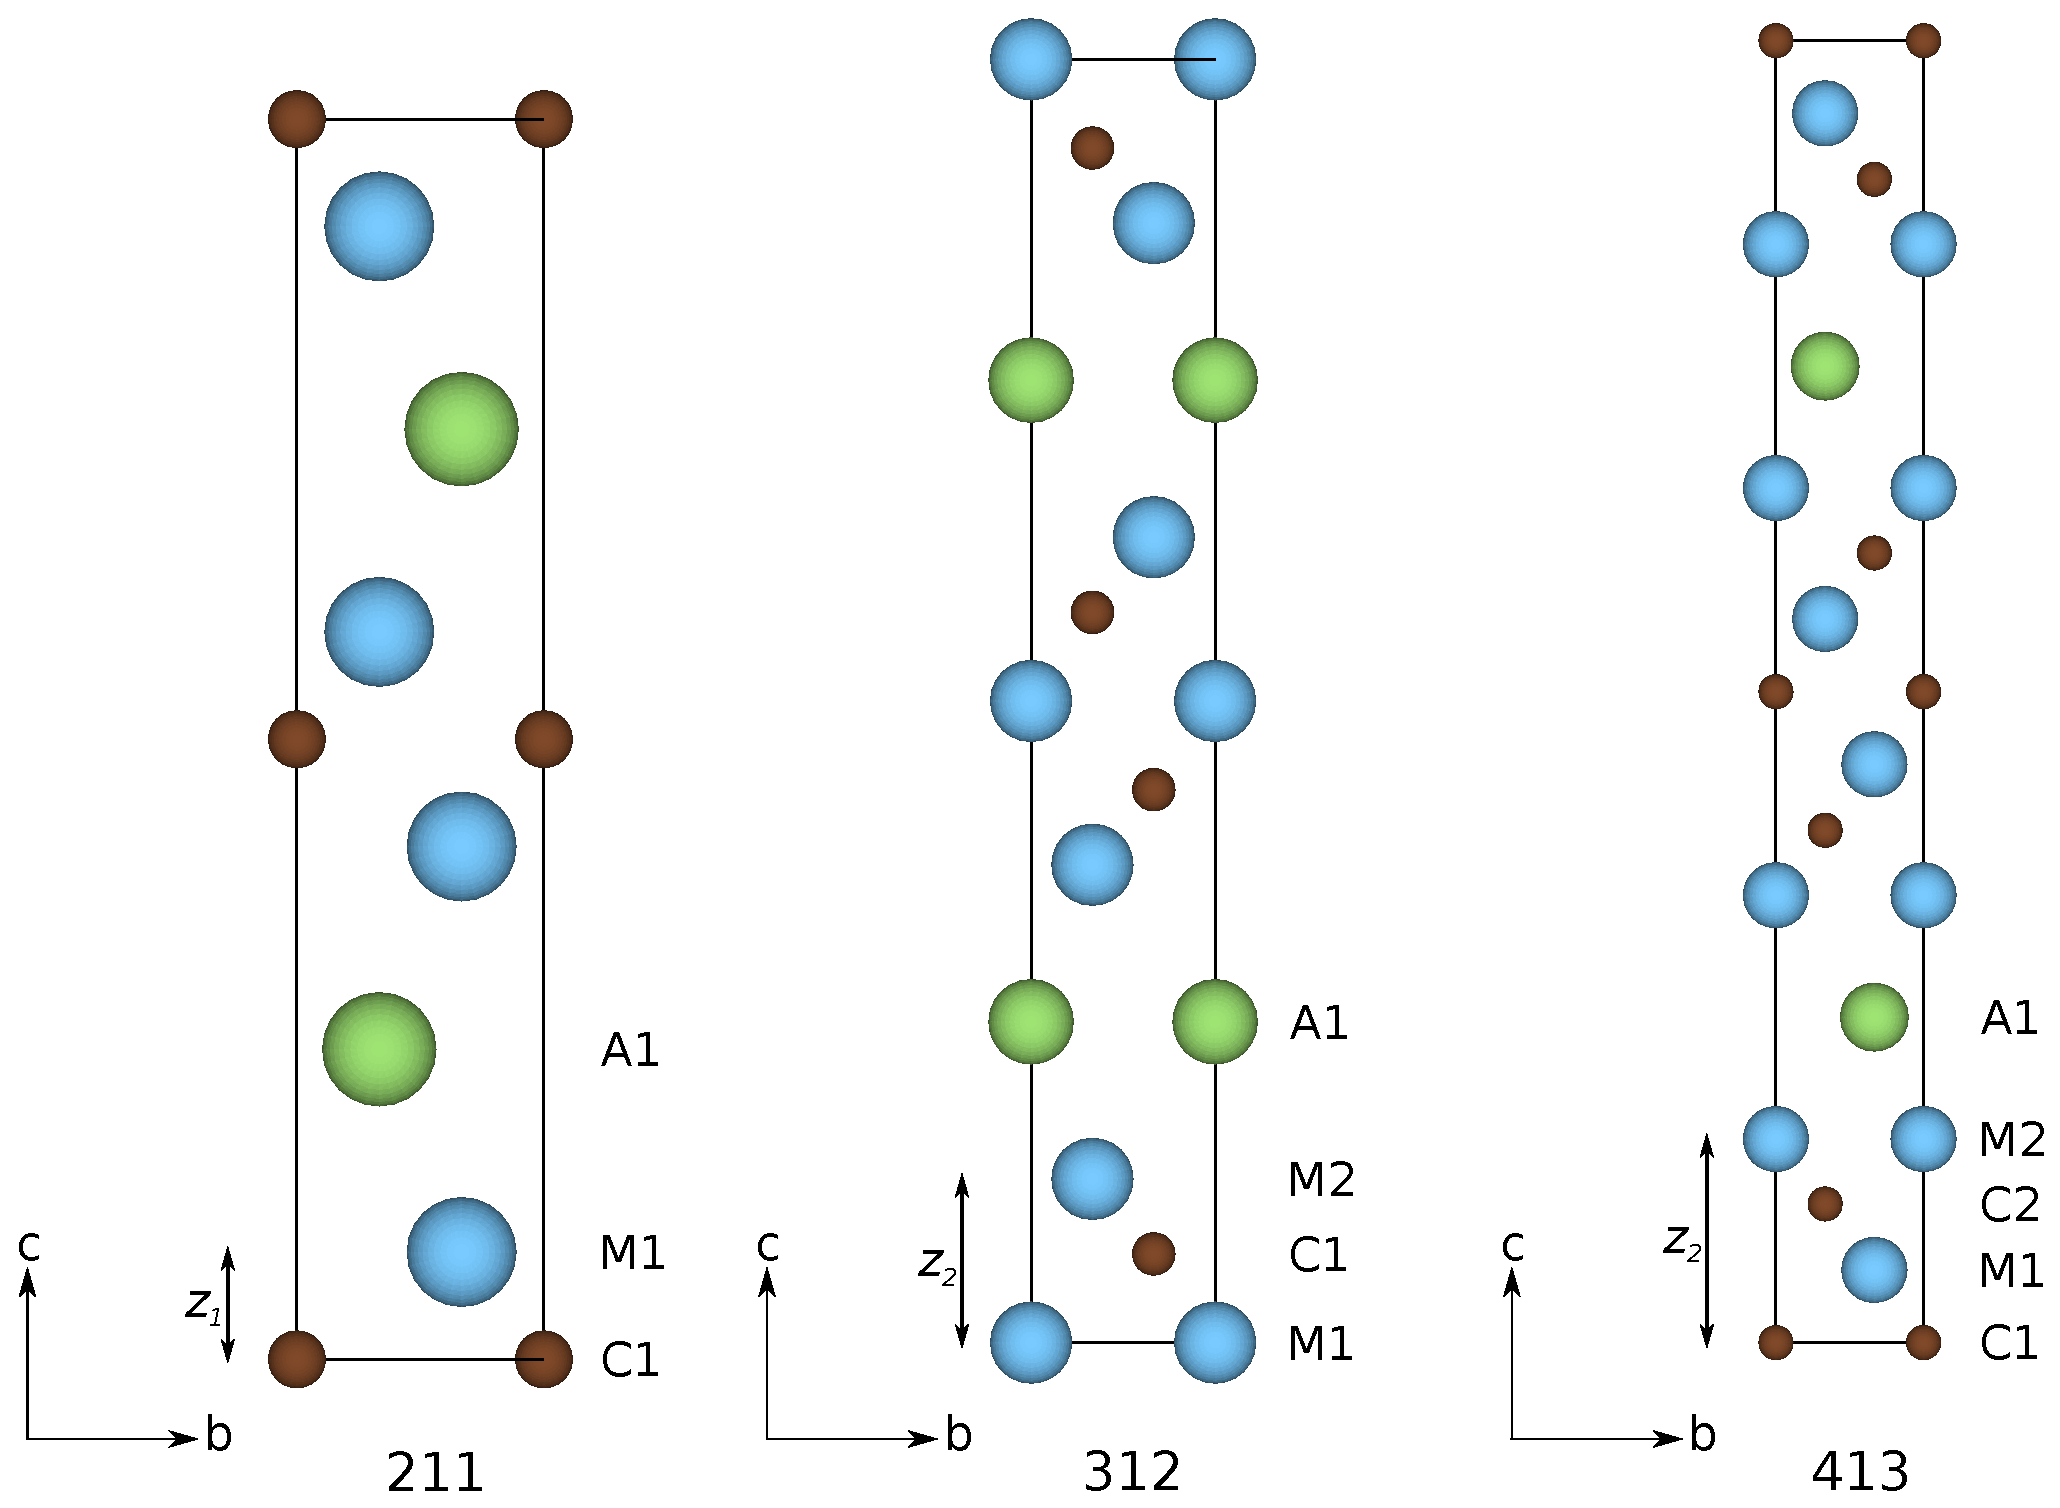
\includegraphics[width=\textwidth]{MAX_unit_cells}
\caption[The MAX phase unit cells.]{The unit cells of the first three possible MAX phases. Graphics prepared with VESTA \cite{Momma2011}.\label{fig:MAX_unit_cells}}
\end{figure}




\begin{figure}
\centering
\captionsetup{width=0.6\textwidth,font={sf,scriptsize},labelfont=bf}
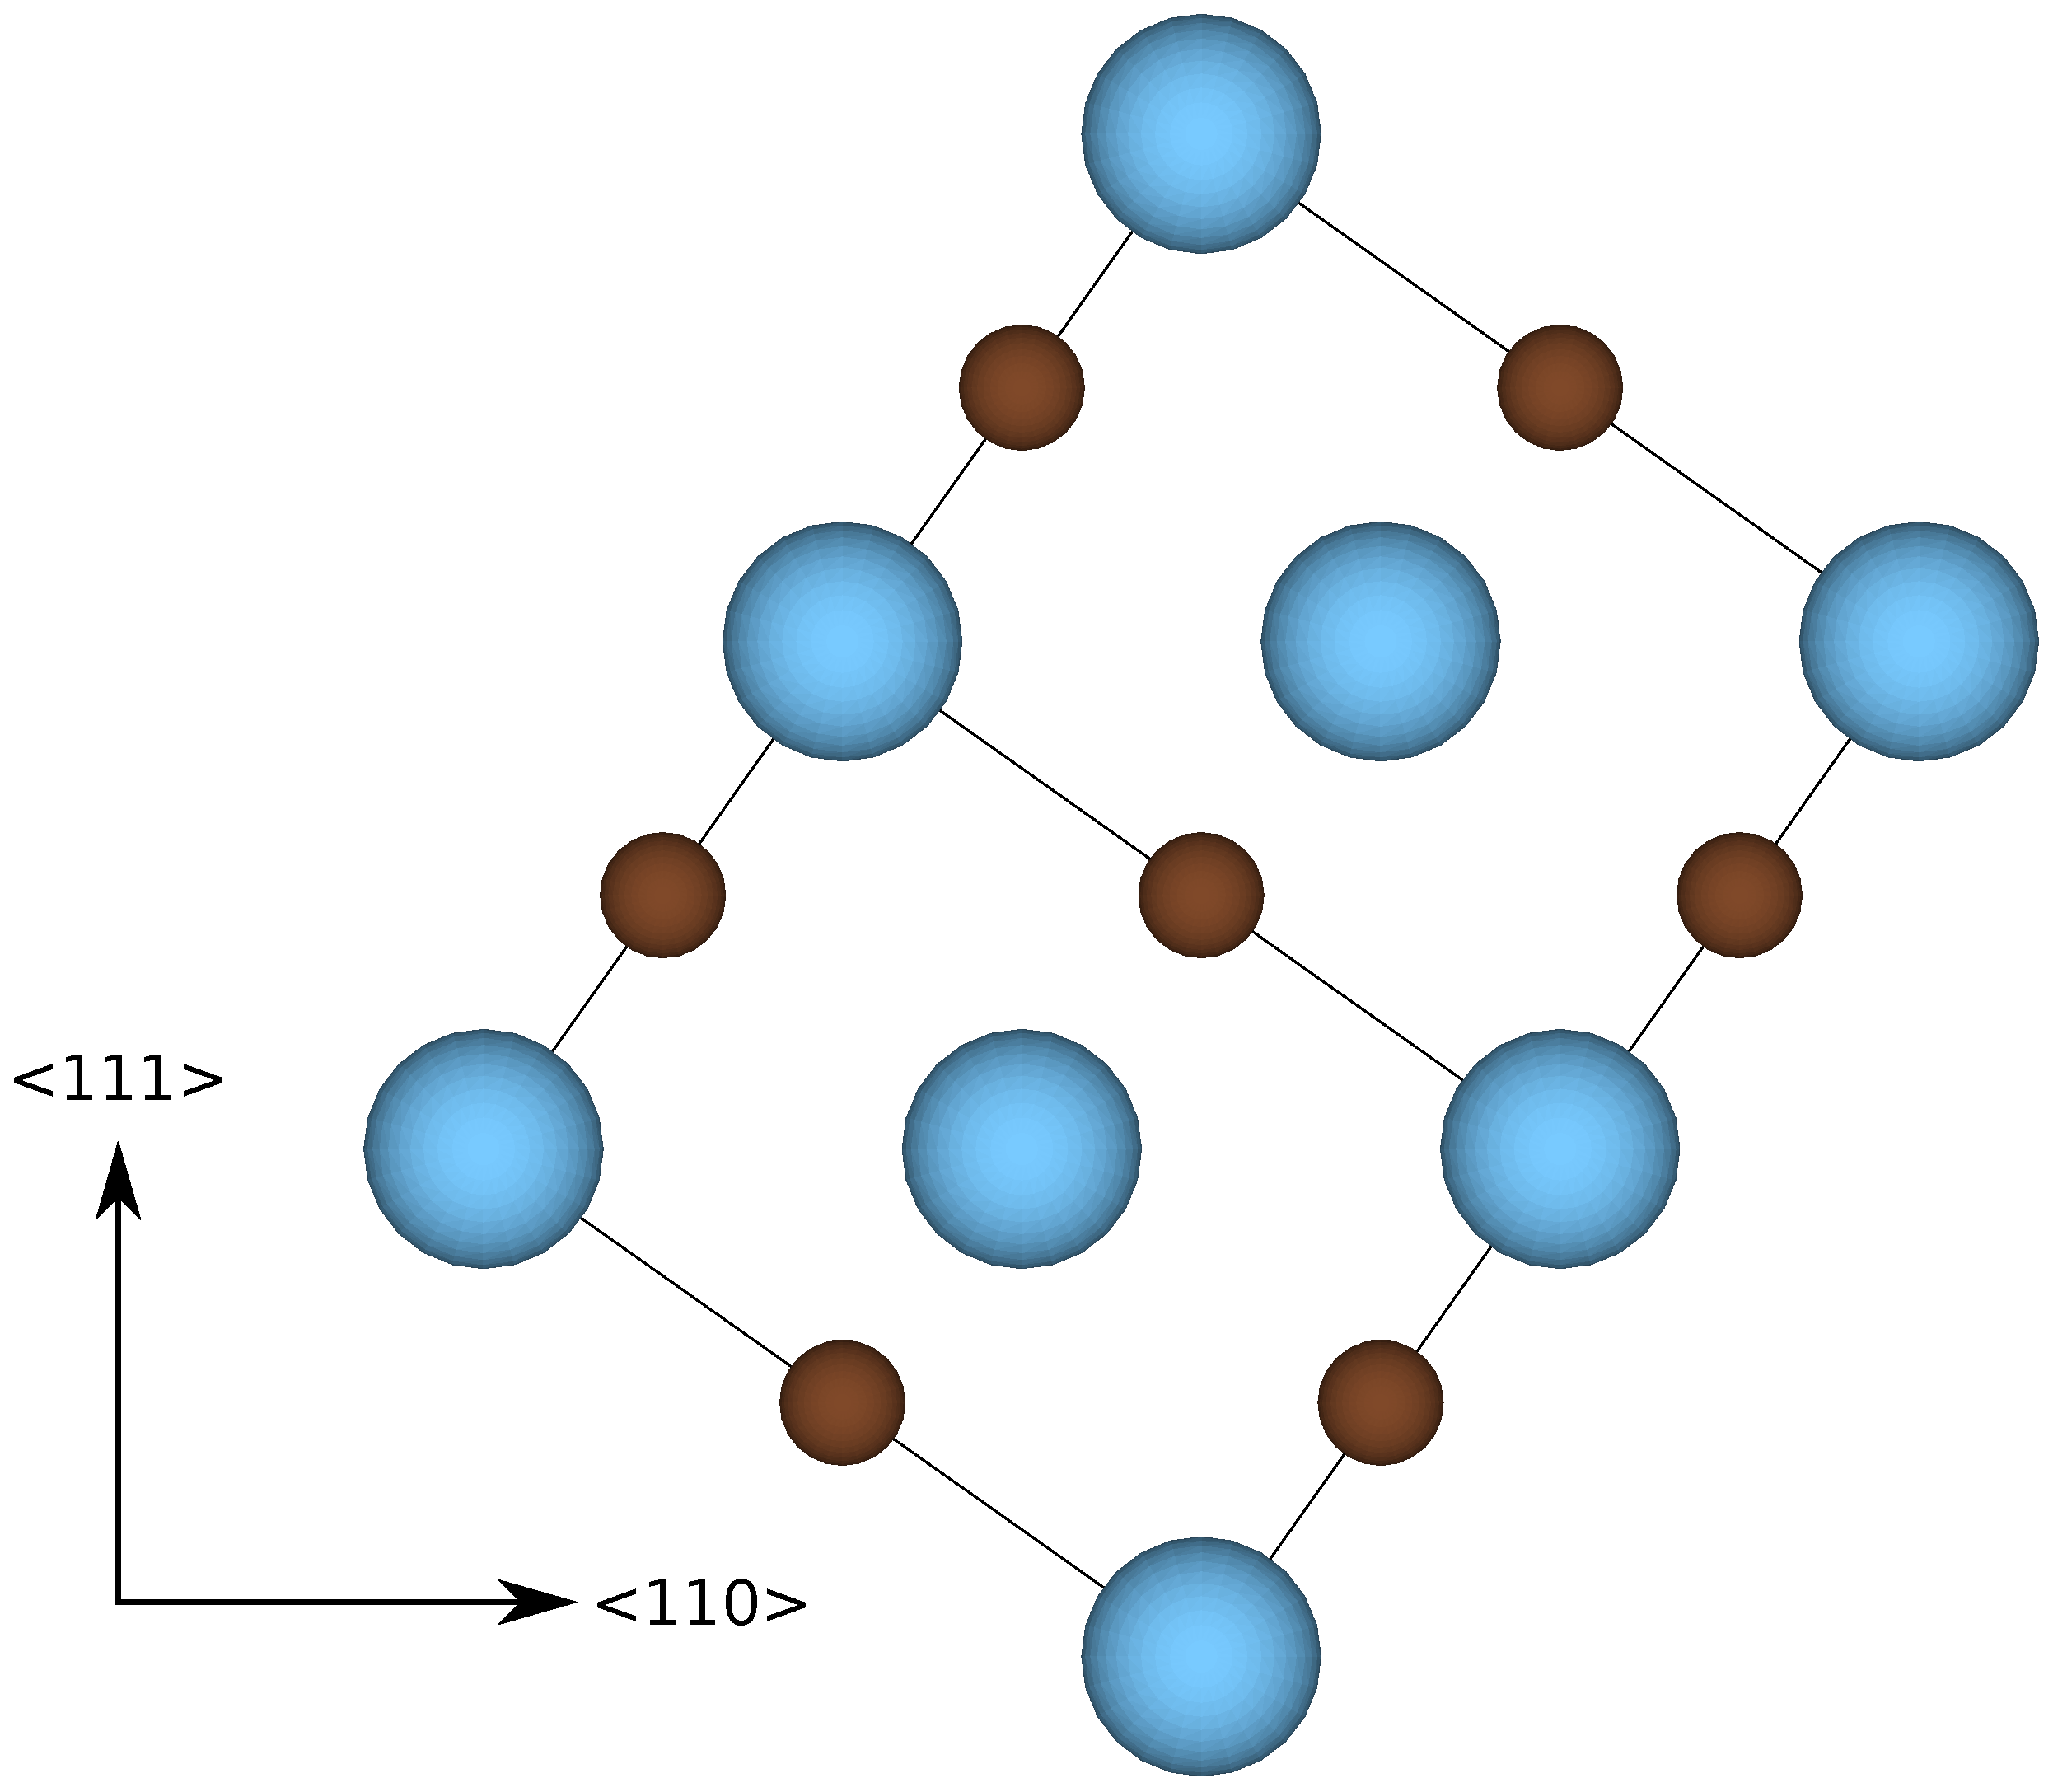
\includegraphics[width=0.5\textwidth]{TiC_111}
\caption[The unit cell of \ce{TiC}.]{The unit cell of \ce{TiC}, which has the rock salt structure, oriented to show the \{1\,1\,1\} planes which are equivalent to the MX layers of the MAX structure shown in \autoref{fig:MAX_unit_cells}. Graphic prepared with VESTA \cite{Momma2011}.\label{fig:TiC_111}}
\end{figure}


The description of complex crystals is often in terms of clusters of atoms that appear to pack together and fill space. The clusters may or may not have physical significance: for example clusters of up to 55 atoms of \ce{Ni}-\ce{Al} are stable on surfaces and so are clearly physically significant, but geometric descriptions of clusters can be made of simple materials like FCC aluminium \cite{Steurer2006}. Care must be taken therefore not to ascribe undue significance to purely geometric features, but the description of the MAX crystal structure as layers is not simply geometric but can be justified on the basis of heterogeneity in the chemical environments, i.e. the layers are meaningful.

The bonding in MAX phases has been shown, by density functional theory (DFT) calculations, to be a combination of metallic, covalent and ionic bonding but with covalent bonding predominant in the MX layer and metallic bonding in MA layers. Large variations in structural and mechanical properties are observed to depend on changes in the nature of this heterogeneous bonding character \cite{Radovic2013,Sun2011}. Notably the extreme (among MAX phases) properties of \ce{Ti2SC} are ascribed to the unusual strong bonding between \ce{Ti} and \ce{S} in addition to the strong bonding between \ce{Ti} and \ce{C} in contrast with most other MAX phases. This unusual bonding is taken to underlie the high elastic constants, $E =$~\SI{316}{\giga\pascal} the highest of any 211 MAX phase, and hardness of \SI{8}{\giga\pascal}, very nearly the highest of any bulk MAX phase \cite{Feng2010,Sun2011}.

\subsection{Deformation in MAX phases}

Deformation in \ce{Ti3SiC2} has been widely studied, particularly by Barsoum \cite{Farber1998,Barsoum1999,Farber1999,Barsoum1999dislocs_kinkbands,Barsoum2001}, and was found to readily occur by the glide of dislocations. Room temperature deformation was shown to increase the density of perfect basal dislocations with a Burgers vector equal to the lattice parameter $a$, so $b =$~<1\,1\,\={2}\,0>. 

Using heavily textured bulk samples of \ce{Ti3SiC2} the critical resolved shear stress of \ce{Ti3SiC2} was estimated by compression test. A sample with the basal planes of the sample oriented at approximately \SI{65}{\degree} to the compression axis and a yield stress of \SI{200}{\mega\pascal} was measured. Schmid's law is 

\begin{equation}
\tau_y = \sigma_y \cos{\phi} \cos{\lambda}
\end{equation}

where $\tau_y$ is the shear yield stress on the slip plane in question, $\sigma_y$ is the uniaxial yield stress\ $\phi$ is the angle between the slip plane normal and the loading axis, and $\lambda$ is the angle between the slip direction and the loading axis. The $\phi$ must be \SI{25}{\degree} ($=\SI{90}{\degree} - \SI{65}{\degree}$) but $\lambda$ is not known but if taken to be the maximum possible value, given $\phi=\SI{25}{\degree}$, of \SI{115}{\degree} then $\tau_y = \SI{77}{\mega\pascal}$, providing an upper bound \cite{Humphrey2012}. While this is higher than the estimate made by the original authors \cite{Barsoum1999}, \citet{Humphrey2012} points out that this is likely an overestimate due to the variation in Schmid factor across the sample and load redistribution between soft and hard grains but in any case is very low for a ceramic and approaches the flow stresses of pure cubic close-packed metals.


%%%%%%%%%%%%%%%%%%%%%%%%%%%%%%%%%%%%%%%%%%%%%%%%%%%%%%%%%%%%%%%%%%
%
%
%
%
%
%
% Figure about compression test here?
%
%
%
%
%
%
%%%%%%%%%%%%%%%%%%%%%%%%%%%%%%%%%%%%%%%%%%%%%%%%%%%%%%%%%%%%%%%


As discussed in \autoref{sec:tailor_peierls}, attempts have been made to explain and hence control the lattice resistance of materials, and this has been done for the MAX phases too. One study on MAX phases \cite{Music2007ductility} with the chemistry \ce{M2AlC} (M = Ti, V, Cr) used the more recent ductility criteria, namely Zhou-Carlsson-Thomson \cite{Zhou1994} and Rice \cite{Rice1992} which are discussed in detail in \autoref{sec:ductility_criteria}. There is recognition that the lattice resistance of a single dislocation, which is the limiting factor on ductility in most ceramics, is not simply dependent on bulk elastic constants. The authors therefore calculate ductility criteria based on stacking fault energies and surface energies, which necessitates choosing which plane to fault or cleave. In the MAX phases there are two natural choices: between the M atom and the A atom or between the M atom and the X atom. However there is no direct link, in these studies, between these properties and dislocation behaviour, and hence no direct link to the ductility. 

Some studies have considered the Peierls stress in complex crystals with layered structures \cite{Music2008,Emmerlich2009,Gouriet2015} but usually these have simply applied the result for an isotropic elastic material:
\begin{equation}
\tau_p = \frac{2G}{1-\nu} \exp \left( - \frac{2 \pi d}{b(1-\nu)} \right)
\end{equation}
where $G$ is the shear modulus, $\nu$ is the Poisson ratio, $d$ is the slip plane spacing and $b$ is the Burgers vector.


The result is therefore based on polycrystalline bulk elastic properties and the specifics of the MAX crystal structure are disregarded save the values of $d$ and $b$ chosen. These have tended to give high values of the Peierls stress, e.g. \SI{980}{\mega\pascal} for \ce{Ti2AlC} \cite{Music2008} which we can compare with \SI{700}{\mega\pascal} for \ce{TiC} \cite{Clegg2006}. The strength of \ce{TiC} should be an upper bound on the flow stress in the MAX phase, since the MAX phases contain planes of \ce{TiC}. Furthermore these planes of TiC in the MAX phases are equivalent to the slip planes in \ce{TiC} \cite{Hollox1966}. 

The GSF calculated by DFT has been used in at least one study \cite{Gouriet2015} but assumed that no change in confining elastic field occurred during dislocation motion, which has been shown to be significant \cite{Lubarda2007,Clegg2006}. \citet{Gouriet2015} also found Peierls stresses that are more similar to \ce{TiC}, of between \SI{611}{\mega\pascal} and \SI{957}{\mega\pascal}.

There is clearly a large effect of the crystal chemistry on the lattice resistance of the MAX phases which has not been adequately explained. If the effect can be understood it may allow a general route to tailoring the Peierls stress of a material and the introduction of a degree of ductility and toughness to otherwise brittle materials.



























































\section{Alternative energy formulations}

\label{sec:empirical_potentials}



The Peierls model is based on a linear elastic formulation of the energy, perhaps with a fitted misalignment potential. Other formulations might provide more insight. Empirical potentials have been developed for a wide range of materials and conditions for the field of molecular dynamics and are tractable computationally while hopefully retaining enough fidelity to actual behaviour to give physical insight \cite{martinez2013}.

Various potentials exist for different types of materials, which usually are applicable to only some classes of materials. For example, the embedded atom method applies well to metals \cite{Daw1984}, the Lennard-Jones and Buckingham potentials describe dispersion interactions, and the short range exchange interaction arising from Pauli exclusion \cite{Jones1924,Buckingham1938} and bond order potentials describe covalent bonding, e.g. the Tersoff potential \cite{Tersoff1988}. 


Ionic solids are an ideal class of materials with which to demonstrate the application of alternative energy calculations by applying empirical potentials. Some modelling of dislocation motion by the conventional Peierls-Nabarro model, using the elastic properties and the generalised staking fault energy, has been undertaken for \ce{MgO} \cite{Miranda2005}, however the chemical bonding is well described by fairly simple empirical potentials that could provide more insight into the factors controlling plasticity than linear elasticity. 

There are large numbers of ionic solids with the same simple crystals structures, e.g. rock salt and caesium chloride \cite{Kelly2012app7}, and the primary contribution to the energy of these materials is the electrostatic interaction, which is mathematically simple:
\begin{equation}
U^{\text{electro}}_{ij} = \frac{1}{4\pi\epsilon_0} \frac{q_i q_j}{r_{ij}}
\end{equation}
where $\epsilon_0$ is the permittivity of free space, $q_i$ is the charge on atom $i$ and $r_{ij}$ is the separation between atoms $i$ and $j$.


The Lennard-Jones potential is often used to capture the shorter range interaction in ionic solids. The Lennard-Jones is one of the simplest formulations to represent these interactions in ionic solids and has the form
\begin{equation}
\phi_{ij}(r_{ij}) = 4\epsilon_{ij} \left[ \left( \frac{\sigma_{ij}}{r_{ij}}\right)^{12}-     \left( \frac{\sigma_{ij}}{r_{ij}}\right)^6   \right]
\end{equation}
or in the ``A--B'' form
\begin{equation}
\phi_{ij}(r_{ij}) = \frac{A_{ij}}{r_{ij}^{12}} - \frac{B_{ij}}{r_{ij}^{6}}
\end{equation}
where $r_{ij}$ is the atomic separation, $\epsilon_{ij}$ is the depth of the energy minimum, $\sigma_{ij}$ is the atomic separation at which the energy is zero and $A_{ij}$ and $B_{ij}$ are simply parameters to be fitted and are related to $\epsilon_{ij}$ and $\sigma_{ij}$ by $A_{ij} = 4\epsilon_{ij}\sigma_{ij}^{12}$ and $B_{ij} = 4 \epsilon_{ij} \sigma_{ij}^{6}$. The total energy for a pair of atoms is then
\begin{equation}
U_{ij}(r_{ij}) = \frac{1}{4\pi\epsilon_0} \frac{q_i q_j}{r_{ij}} + \frac{A_{ij}}{r_{ij}^{12}} - \frac{B_{ij}}{r_{ij}^{6}}
\end{equation}




The energy of perfect ionic crystals is relatively easily calculated  via a Madelung or Ewald summation \cite{madelung1918,Ewald1921}, but these usually rely on an assumption of symmetry; an assumption that is broken by the introduction of a defect. In the case of a dislocated crystal another approach is required. One option is a direct sum, which scales with the square of the number of atoms in the simulation. If the distance from the dislocation line is considered the simulation time scales with the fourth power, which can rapidly become intractable. However advances in computing hardware and efficient implementations of array operations in NumPy \cite{Numpy2011}, particularly an efficient implementation of the Einstein summation convention \cite{opt_einsum} may make this a workable solution.


An alternative is to use an implementation of a long range electrostatics solver that allows for non periodicity in two dimensions. One such implementation is the multiscale summation method in LAMMPS \cite{Hardy2009,Plimpton1995,LAMMPS_web}, which divides the problem into one short range potential plus a series of smoothly vanishing long range potentials over increasingly coarse meshes at larger interatomic distances. The use of LAMMPS allows the extension of the energy calculations to other energy terms such as polarisability of ions and so on.


\subsection{Dislocations in ionic crystals}




The rocksalt structure is particularly common in ionic solids and phases of this structure have been widely studied in terms of their plasticity. The slip direction is usually <1\,1\,0> and the active slip planes are \{0\,0\,1\} and \{1\,\={1}\,0\}, and sometimes \{1\,\={1}\,1\}. For edge dislocations the last would expose charged surfaces of atoms at free surfaces, so despite being the closest packed plane it is not commonly seen \cite{Haasen1985}. Schematic illustrations of edge dislocations are shown in \autoref{fig:Schematic_NaCl_dislocs}.

\begin{figure}
\centering
    \begin{subfigure}{0.8\textwidth}
    \centering
    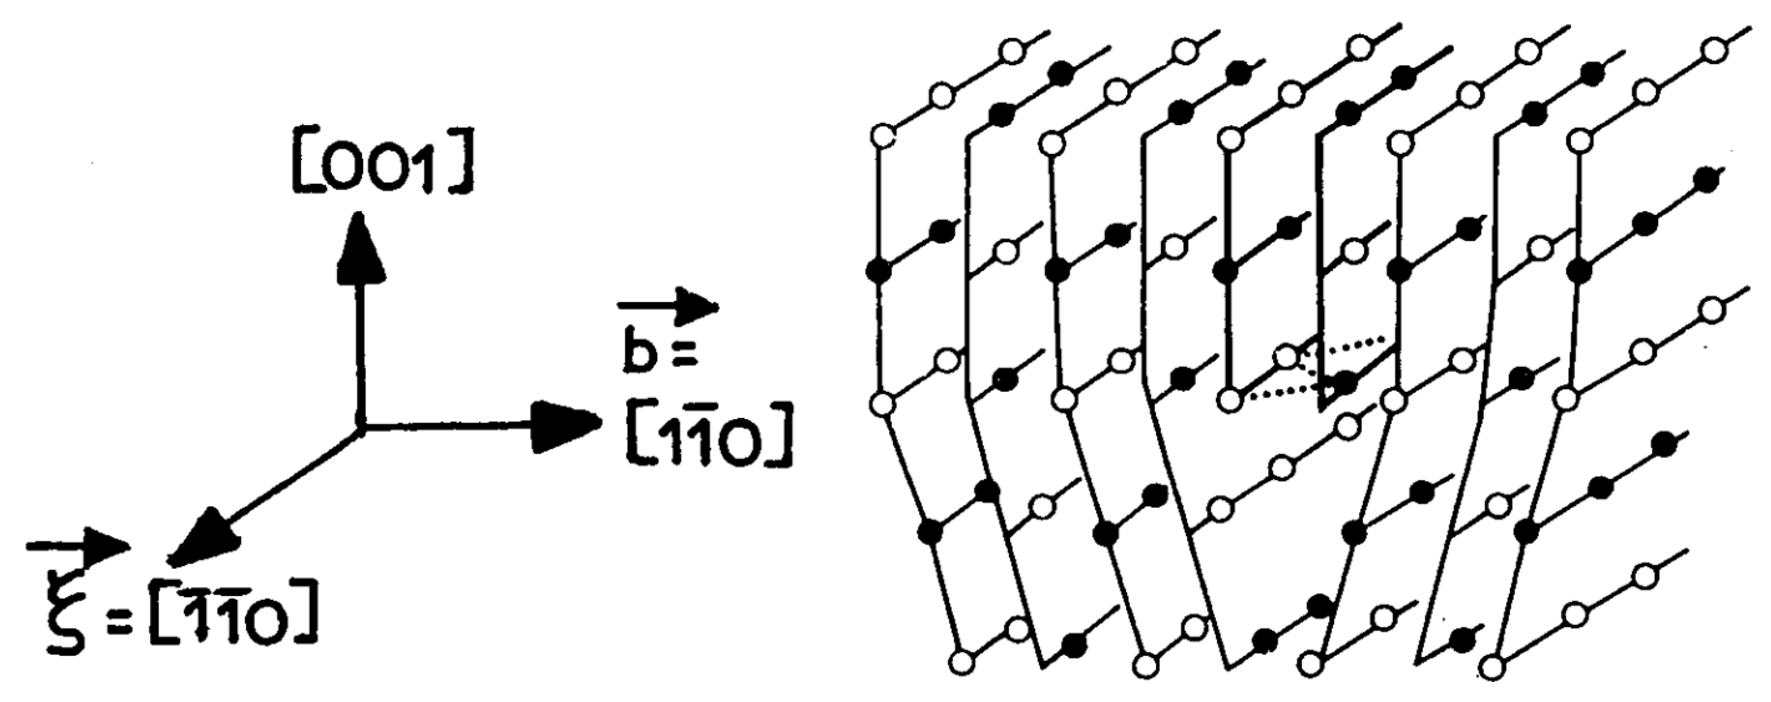
\includegraphics[width=\textwidth]{NaCl_001_1-10}
    \caption{The \{0\,0\,1\}<1\,\={1}\,0> slip system.\label{fig:NaCl_110_001_core_structure}}
    \end{subfigure}
\par\bigskip
    \begin{subfigure}{0.8\textwidth}
    \centering
    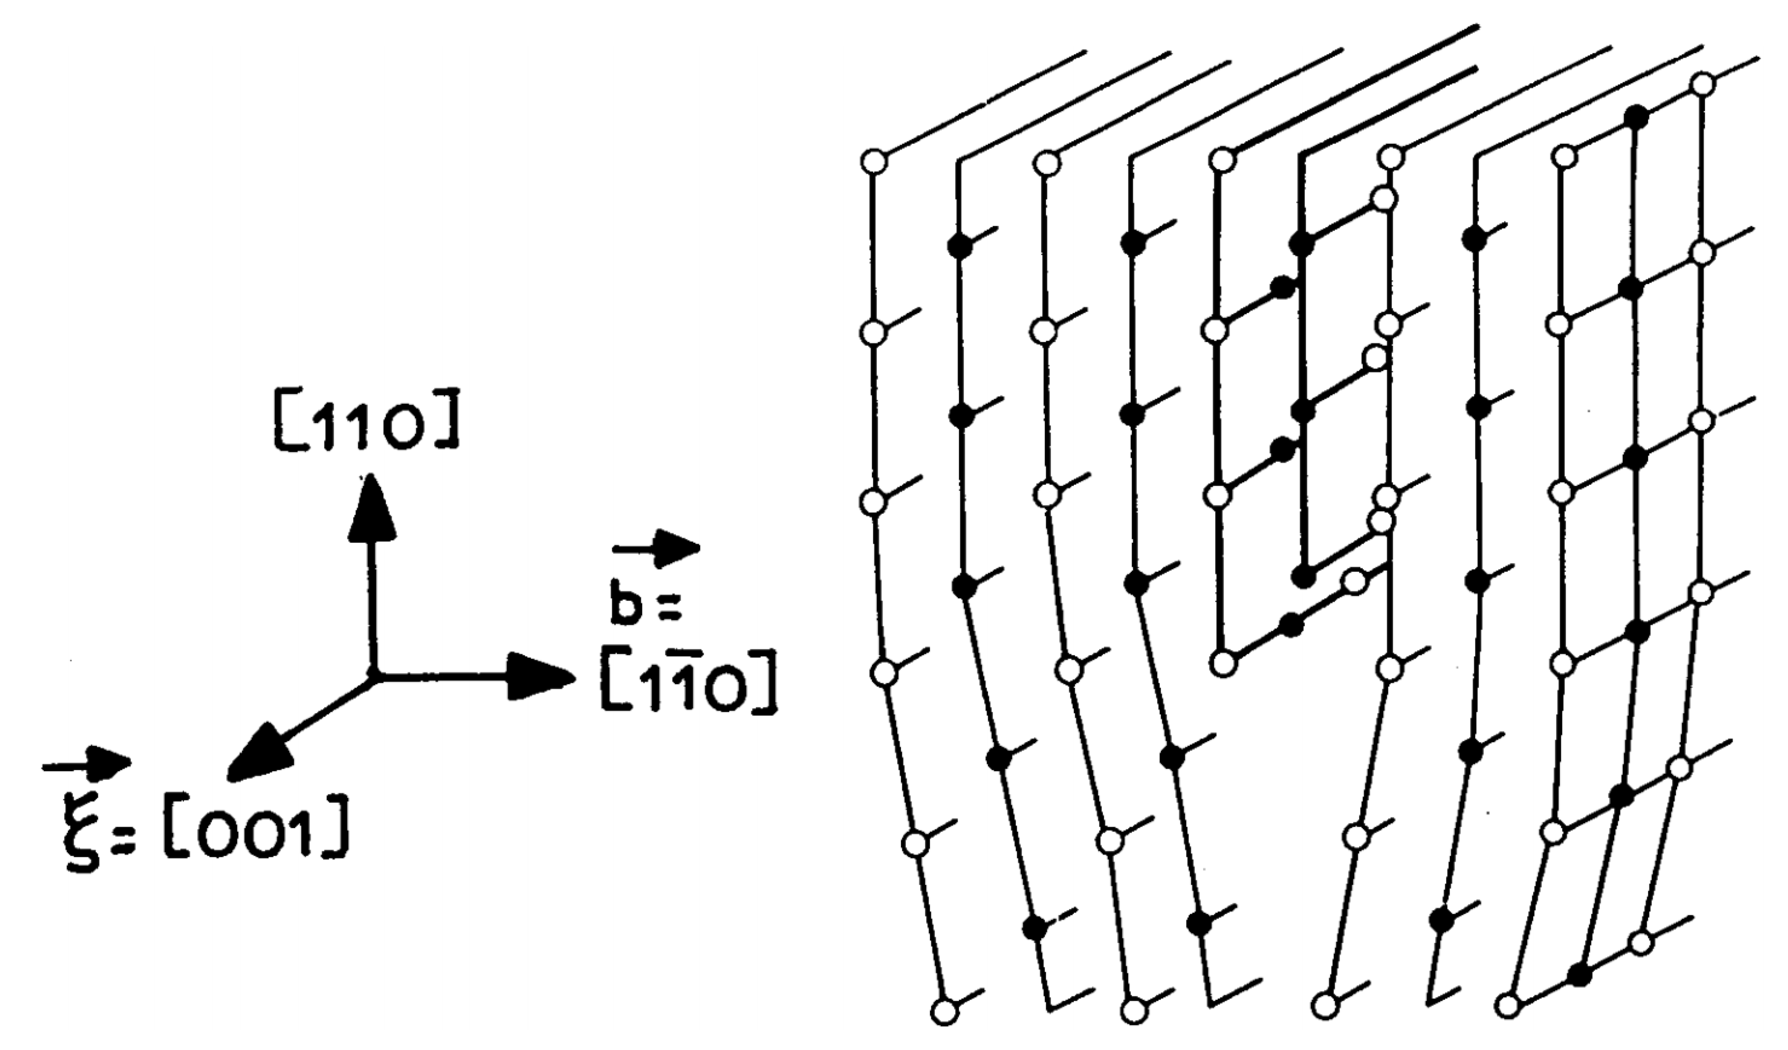
\includegraphics[width=\textwidth]{NaCl_110_1-10}
    \caption{The \{1\,1\,0\}<1\,\={1}\,0> slip system.\label{fig:NaCl_110_110_core_structure}}
    \end{subfigure}
\caption[Edge dislocations in the rock salt crystals.]{Schematic edge dislocations in the rocksalt structure reproduced from \cite{Haasen1985}. \label{fig:Schematic_NaCl_dislocs}}
\end{figure}





Experimental work has characterised the yield stress of ionic solids with the rocksalt structure over a wide range of temperatures, including very low temperatures by using liquid helium (\SI{\sim4}{\kelvin}), and they deviate strongly from the prediction of elastic Peierls models. This makes them useful as a model system for testing dislocation theories \cite{Haasen1985}.

Previous modelling of dislocations in ionic crystals has been undertaken, notably by \citet{puls1976} who simulated edge \{0\,0\,1\}<1\,\={1}\,0> dislocations in \ce{MgO}, and by \citet{Woo1977} who modelled the same dislocation geometry in a range of ionic crystals with the rocksalt structure, among others \cite{Granzer1968,Woo1976,Hoagland1976,Brandt1987,Soullard1991,Foitzik1991}. These were limited by the computational resources available and used a variety of strategies to overcome these limits; one approach was to optimise only the equilibrium position and then assume linear trajectories for the atoms for intermediate states, as developed by \citet{Granzer1968}. This is similar to the assumption made by Peierls \cite{Peierls1940} that the dislocation width does not vary between the equilibrium positions, which has been shown to have a very large effect on the results \cite{Clegg2006,Bulatov1997}.

Another method to overcome computational limitations was to simulate only small regions atomistically. This was achieved by applying a variety of boundary conditions, usually derived from elasticity theory, to constrain the atomistic region and modelling material outside this core region as elastic. Such conditions were used in \cite{Woo1977}. The use of conditions like these prevents the separation of the different energetic components since there is always a large contribution from the elastic region as well as the electrostatics and short-range interactions. A fully atomistic simulation would hopefully show the individual energy contributions and give some insight into the dominant factors  controlling dislocation motion.

A fully atomistic model using suitable interatomic potentials will hopefully illustrate the factors that control dislocation motion in ionic solids.



























































































































